\documentclass{article}
\usepackage{graphicx} % Required for inserting images
\usepackage[margin=2cm, top=3cm]{geometry} % margine superiore ridotto a 1 cm
\usepackage{listings}
\usepackage{subcaption}  % Pacchetto per sottodidascalie
\usepackage{float}       % Pacchetto per posizionamento rigido delle figure
\title{Sistemi Operativi}
\author{Mattia Cosimi}
\date{October 2024}

\begin{document}

\maketitle

\section{Introduzione ai sistemi operativi}
Un programma in esecuzione esegue istruzioni. \\
Il processore recupera un’istruzione dalla memoria,\\
La decodifica,\\
La esegue,\\
Successivamente si sposta sulla prossima istruzione (Modello di Von Neumann).\\
\subsection{Di cosa si occupa il sistema operativo?}
Il sistema operativo è responsabile di rendere semplice l’esecuzione di programmi, permettere ai programmi di condividere la memoria, permettere ai programmi di interagire con gli altri dispositivi. Il sistema operativo ha il compito di controllare che il sistema lavori in modo efficiente e corretto. Il sistema operativo prende una risorsa fisica e la trasforma in una virtuale. Sostanzialmente grazie alle chiamate di sistema permettiamo all’utente di dire cosa fare al sistema operativo. Quindi un sistema operativo gestisce le risorse, condivisione della cpu e condivisione delle memorie. Il sistema operativo virtualizzando la cpu ci da l’impressione che questa utilizzi un numero infinito di cpu (Guarda cpu.c). Per quanto riguarda la virtualizzazione della memoria la memoria viene letta: specificando un indirizzo dove accedere ai dati e viene scritta: specificando i dati da scrivere all’indirizzo evocato (Guarda mem.c). Nella virtualizzazione della memoria ogni processo accede al suo spazio di indirizzi virtuali privati. Il sistema operativo mappa lo spazio degli indirizzi sulla memoria fisica. La memoria fisica è una risorsa condivisa gestita dal sistema operativo. Un altro problema è quello della concorrenza dato dai programmi multi thread. Si può immaginare che il nostro programma segua un filo principale e che durante l’esecuzione di possano creare dei nuovi fili secondari (Guarda threads.c). Quando in un programma abbiamo il semplice incremento di una variabile, in realtà stiamo eseguendo tre istruzioni: caricare il valore della variabile dalla memoria al registro, incrementarla e rimetterla nella memoria; Queste tre istruzioni non vengono eseguite atomicamente, vengono infatti considerate non un'unica istruzione ma tre diverse. Persistenza, hardware e software devono essere in grado di contenere dati persistentemente (file, dati…), Il sistema operativo si occupa di capire dove andranno messi i nuovi dati, infatti emette delle richieste al dispositivo di archiviazione sottostante. I goal del sistema operativo sono quindi: costruire un astrazione e quindi rendere il sistema semplice da utilizzare, fornire delle buone performance, protezione tra le applicazioni e essere affidabile.
\subsection{Il processo di astrazione}
\paragraph{Processo: applicazione in esecuzione (Un’applicazione è un insieme di istruzioni su un qualche dispositivo di archiviazione).}
Il meccanismo che ci permette di eseguire più programmi con poche cpu è il time sharing, consiste nell’assegnare un’unità di tempo (quanto) a un processo, quando questa porzione di tempo finisce ho due opzioni 1. Finisco il processo che stavo eseguendo e passo a un altro 2. Non sono riuscito a finire il processo lo blocco momentaneamente per passare a un altro. Il meccanismo di stoppare un processo e passare a un altro viene detto context switching. Ovviamente il context switching è basato su alcune policy che prendono la decisione su quando stoppare un processo per quanto ecc… Tornando ai processi un processo è composto da la parte della memoria come istruzioni e dati e la parte dei registri come program counter e stack pointer. Il sistema operativo si occupa di controllare il ciclo di vita dei processi, lo fa con le seguenti funzioni: lo crea, lo distrugge, può metterlo in stato di wait, gli fa i vari controlli e ottiene informazioni sullo stato del processo. Riguardo invece alla creazione di un processo: viene caricato il codice di un programma nella memoria, nello spazio degli indirizzi di un processo, si dice che il sistema operativo carica i processi in maniera “pigra” (Per ottimizzare l’utilizzo della memoria si carica il minimo indispensabile nella memoria e poi quando le funzioni vengono richieste viene allocata ulteriore memoria). Viene allocato lo stack a tempo di esecuzione, solitamente lo stack è utilizzato per variabili locali, parametri di funzioni e return address. Viene creato l’heap del programma, utilizzato per i dati allocati dinamicamente (malloc ()), vengono inizializzate le altre cose e successivamente viene fatto eseguire il programma. Un processo può avere tre stati: in esecuzione (running) , pronto (ready): il processo è pronto per andare in esecuzione ma per qualche motivo il sistema operativo ha deciso di non eseguirlo in questo momento, bloccato (blocked). Il sistema operativo ha delle strutture dati per organizzare le informazioni es. xv6 kernel proc structure. Ritornando al time sharing l’obiettivo del sistema operativo è quello di realizzare il context switching con meno overhead possibile, ovvero tutto quell’insieme di istruzioni che posso evitare di eseguire. Un altro obiettivo è quello di avere, da parte del SO, il controllo di quello che sta succedendo. Alcuni processi hanno bisogno di effettuare operazioni che non tutti potrebbero fare, per questo motivo nasce la problematica dell’implementare un meccanismo che gestisca i permessi di questi processi. La soluzione è stata creare due modelli di lavoro. Uno per i processi regolari che non hanno accesso a tutte le risorse hardware, detto User Mode e l’altro per dei processi particolari che hanno accesso a tutte le risorse detto Kernel Mode. Le chiamate di sistema fanno si che i processi abbiano accesso alle funzionalità della kernel-mode. Per eseguire una chiamata di sistema un programma lancia un istruzione trappola che salta nel kernel e aumenta il livello di priorità a kernel-mode. Dopo quest’istruzione trappola tutto ritorna come prima e il livello di privilegio ridiventa User Mode. Ovviamente dato che saltare da una modalità all’altra sarebbe un pericolo il Kernel ha una Trap table dove un numero è associato a ogni chiamata di sistema. Come fa il sistema operativo a riprendere il controllo della cpu, in modo da poter passare da un processo a un altro: ci sono due approcci, Uno cooperativo (aspettare per le chiamate di sistema) e uno non cooperativo (il sistema operativo prende il controllo). I processi cedono regolarmente la CPU effettuando chiamate di sistema come yield(). Le applicazioni trasferiscono il controllo al sistema operativo quando stanno facendo qualcosa di illegale (divisione per 0). L’utilizzo di questo approccio è spesso meno che ottimale: uno dei motivi potrebbe essere un processo cattivo che propositamente non fa nessuna chiamata di sistema. Per quanto riguarda l’altro approccio al sistema operativo serve che l’hardware sia collaborativo per realizzare un approccio non cooperativo. Timer interrupt: Durante la sequenza di avvio il sistema operativo inizializza un timer, il timer genera un interruzione ogni tot tempo. Quando viene generata un interruzione il processo in esecuzione viene arrestato, lo stato del programma viene salvato, un gestore di interruzioni preconfigurato nel sistema operativo viene eseguito, Questo Timer Interrupt consente al sistema operativo di riprendere l’esecuzione su una CPU. Quando si verifica un Timer Interrupt il sistema operativo si occupa di disabilitare le interruzioni date dal timer e si occupa di utilizzare degli schemi che impediscono l accesso concorrente.
\section{Scheduling}
\subsection{Introduzione allo scheduling}
Abbiamo visto come viene implementato il context switch ma dobbiamo ancora discutere delle policy che si trovano al di sopra di questo meccanismo. Per farlo facciamo delle assunzioni che si discostano dalla realtà: (Queste assunzioni verranno modificate per capire meglio le politiche)\\\\
Ogni job (processo) ci mette lo stesso tempo a essere eseguito, \\
Ogni job arriva nello stesso momento,\\
Una volta iniziato il job dev’essere completato,\\
Tutti i job utilizzano solo la cpu e non I/O,\\
Il tempo di esecuzione di ogni job è noto.\\ \\
Una metrica con cui giudicheremo le varie politiche di scheduling è il Turnaround Time che sarebbe quanto tempo il processo è rimasto nel sistema ovvero \( T_{Turnaround}=T_{Completion}-T_{Arrival} \) con le assunzioni che abbiamo fatto adesso che ogni processo arriva a tempo 0 il Turnaround è uguale al tempo di completamento del processo. Un’altra metrica è “fairness” quanto equamente le risorse vengono divise tra i processi.
\subsection{FIFO/First-In-First-Out o FCFS/First-Come-First-Served}
Implementare una strategia fifo può essere conveniente solo con le nostre assunzioni, infatti se i processi non arrivassero tutti a tempo zero e avessero un tempo di esecuzione differente tra loro il turnaround medio si alzerebbe troppo e si crea quello che viene detto effetto convoglio, se arriva prima il processo più lungo, quelli dopo ne devono aspettare il completamento
\begin{figure}[h] % 'h' per indicare di posizionare la figura qui
    \centering % Centra l'intera figura
    % Immagine di sinistra
    \begin{subfigure}[t]{0.45\textwidth} % Sottotitolo di dimensione 45% della larghezza
        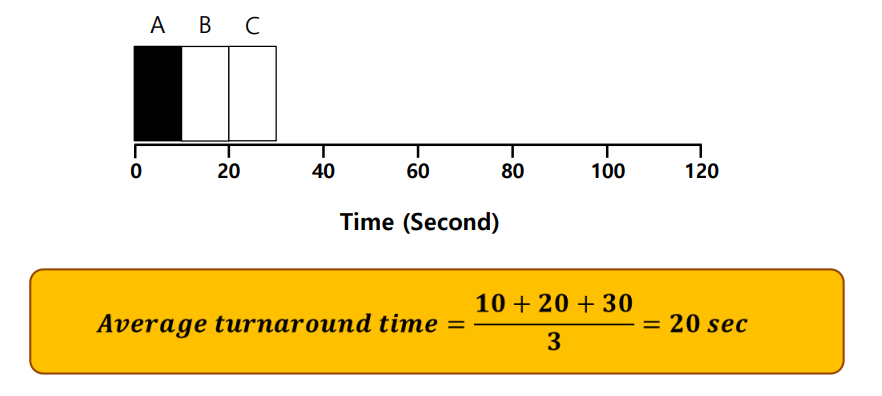
\includegraphics[width=\linewidth]{Screenshots/Screenshot 2024-10-14 173122.png} % Percorso dell'immagine
        \caption{Processi con tempo di esecuzione uguale} % Didascalia per la prima immagine
        \label{fig:sinistra} % Etichetta per riferimento
    \end{subfigure}
    \hspace{0.05\textwidth} % Spazio orizzontale tra le immagini
    % Immagine di destra
    \begin{subfigure}[t]{0.45\textwidth} % Sottotitolo di dimensione 45% della larghezza
        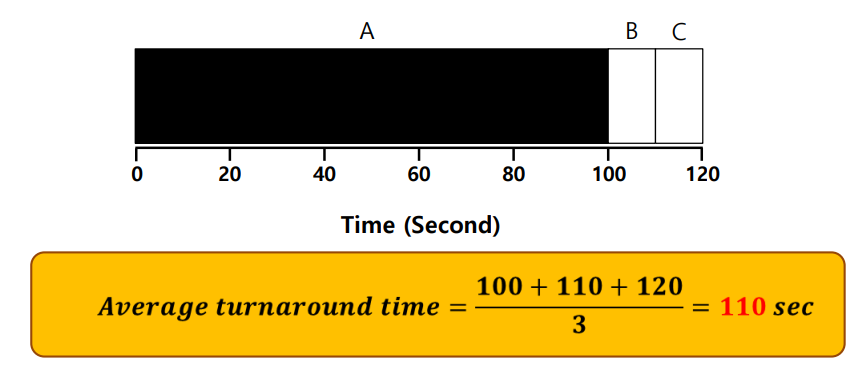
\includegraphics[width=\linewidth]{Screenshots/Screenshot 2024-10-14 173140.png} % Percorso dell'immagine
        \caption{Processi con tempo di esecuzione differenti} % Didascalia per la seconda immagine
        \label{fig:destra} % Etichetta per riferimento
    \end{subfigure}
    \caption{FIFO/First-In-First-Out o FCFS/First-Come-First-Served} % Didascalia generale per la figura
    \label{fig:due_immagini} % Etichetta generale per riferimento
\end{figure}
\subsection{SJF/Shortest Job First}
Come fa intuire il titolo viene eseguito prima il processo più corto poi il secondo più corto e così via. La criticità di questo è simile alla FIFO, in questo caso se è presente un solo processo che è anche il più lungo e ne viene iniziata l’esecuzione e poco dopo arrivano gli altri processi, nuovamente si ritrovano bloccati dal processo più lungo.
\begin{figure}[h] % 'h' per indicare di posizionare la figura qui
    \centering % Centra l'intera figura
    % Immagine di sinistra
    \begin{subfigure}[t]{0.45\textwidth} % Sottotitolo di dimensione 45% della larghezza
        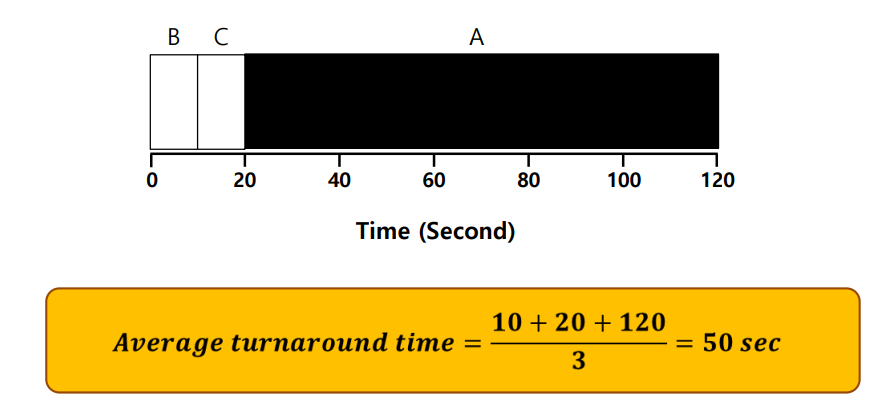
\includegraphics[width=\linewidth]{Screenshots/Screenshot 2024-10-14 173656.png} % Percorso dell'immagine
        \caption{Arrivo in precedenza dei processi più piccoli} % Didascalia per la prima immagine
        \label{fig:sinistra} % Etichetta per riferimento
    \end{subfigure}
    \hspace{0.05\textwidth} % Spazio orizzontale tra le immagini
    % Immagine di destra
    \begin{subfigure}[t]{0.45\textwidth} % Sottotitolo di dimensione 45% della larghezza
        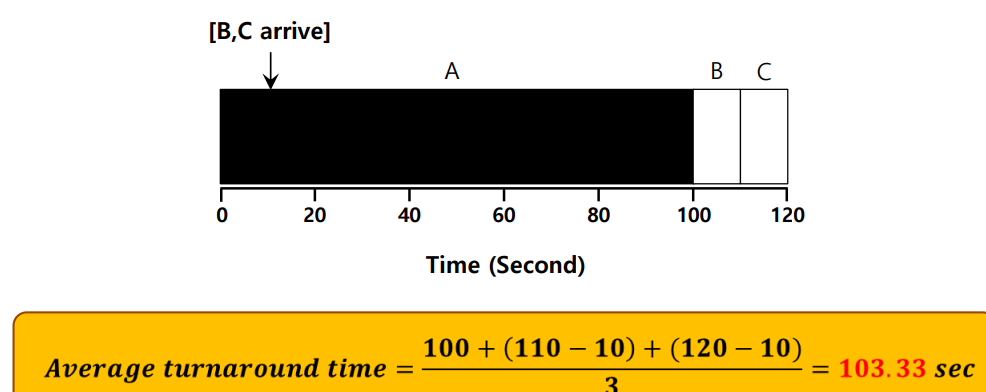
\includegraphics[width=\linewidth]{Screenshots/Screenshot 2024-10-14 173707.png} % Percorso dell'immagine
        \caption{Arrivo in precedenza del processo più grande} % Didascalia per la seconda immagine
        \label{fig:destra} % Etichetta per riferimento
    \end{subfigure}
    \caption{SJF/Shortest Job First} % Didascalia generale per la figura
    \label{fig:due_immagini} % Etichetta generale per riferimento
\end{figure} \\\\\\\\\\\\\\\\\\\\\\\\
\subsection{STCF/Shortest-Time-to-Completion-First}
Questa politica è simile al SJF solo che non si basa sul tempo di esecuzione del processo ma sul tempo di esecuzione rimasto del processo.
\begin{figure}[H] % Usa 'H' per forzare la posizione qui
    \centering % Centra l'immagine
    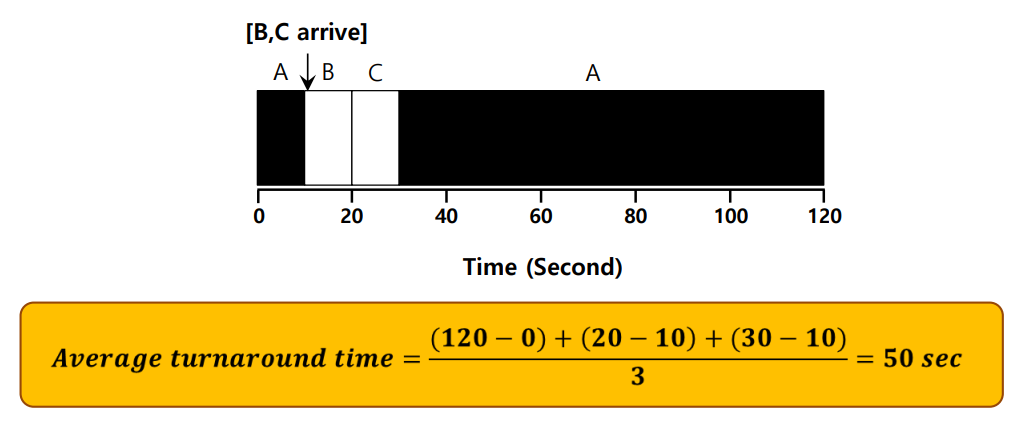
\includegraphics[width=0.8\textwidth]{Screenshots/Screenshot 2024-10-14 174351.png} % Percorso dell'immagine
    \caption{Miglioramento della politica precedente} % Didascalia per l'immagine
    \label{fig:immagine} % Etichetta per riferimento
\end{figure}
\noindent %Per togliere lo spazietto fastidioso
Aggiungiamo un'altra metrica di giudizio che è il tempo di risposta, che consiste nel tempo che quel job è stato in coda prima di eseguire la prima istruzione ed è uguale a \( T_{Response}=T_{Firstrun}-T_{Arrival} \)
\begin{figure}[H] % Usa 'H' per forzare la posizione qui
    \centering % Centra l'immagine
    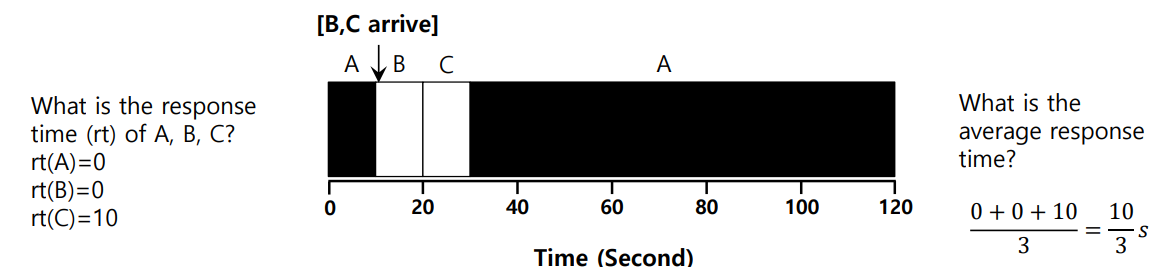
\includegraphics[width=0.8\textwidth]{Screenshots/Screenshot 2024-10-14 174623.png} % Percorso dell'immagine
    \caption{Calcolo del tempo di risposta} % Didascalia per l'immagine
    \label{fig:immagine} % Etichetta per riferimento
\end{figure}
\subsection{RR/Round Robin}
Questa politica è basata su fette temporali, ovvero un job va in esecuzione per un certo quanto di tempo, successivamente viene mandato in esecuzione un altro job fino a che non c’è più nulla in coda. Questa politica è fair ma così facendo ottiene un turnaround pessimo.
\begin{figure}[H] % Usa 'H' per forzare la posizione qui
    \centering % Centra l'immagine
    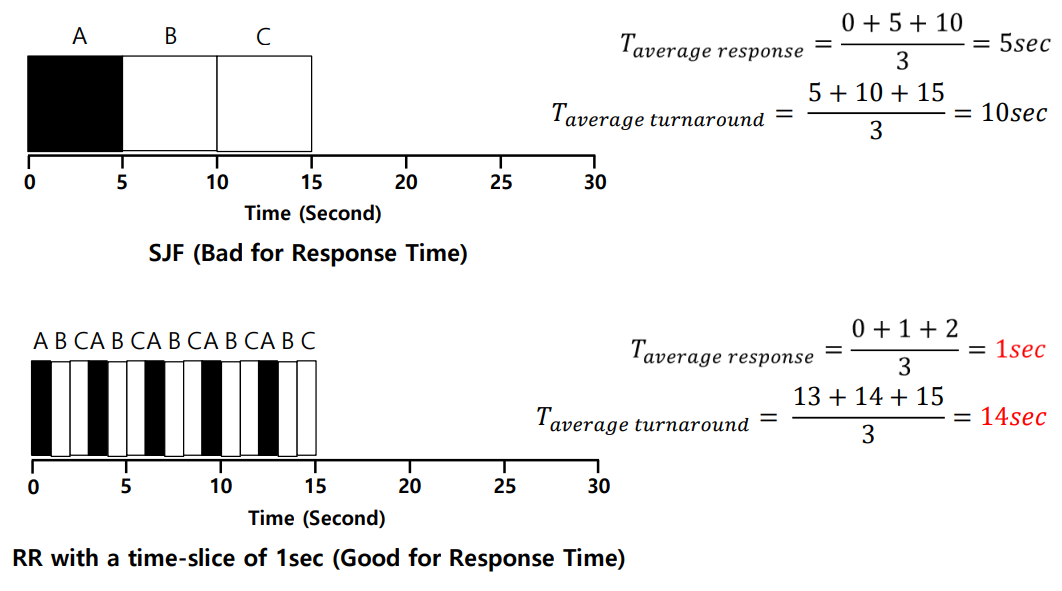
\includegraphics[width=10cm, height=5cm]{Screenshots/Screenshot 2024-10-14 175219.png} % Percorso dell'immagine
    \caption{Ottimo tempo di risposta ma pessimo Turnaround Time} % Didascalia per l'immagine
    \label{fig:immagine} % Etichetta per riferimento
\end{figure}
\noindent %Per togliere lo spazietto fastidioso
Questa politica sia con un quanto di tempo lungo che corto ha sempre delle criticità. Più il quanto di tempo è piccolo e più il costo del context switch dominerà le performance. Più il quanto di tempo è grande e peggiore sarà il tempo di risposta. Generalmente ogni politica fair avrà un cattivo turnaround time. Se volessimo incorporare anche l’I/O dovremmo modificare qualche assunzione, del tipo i processi possono usare I/O, Quando un job inizia una richiesta di I/O: Il job rimane bloccato e aspetta che l’I/O finisca, il gestore dovrebbe gestire un altro job sulla cpu. Quando l’I/O finisce viene sollevato un Interrupt e il sistema operativo modifica lo stato del processo da bloccato a pronto
\begin{figure}[H] % Usa 'H' per forzare la posizione qui
    \centering % Centra l'immagine
    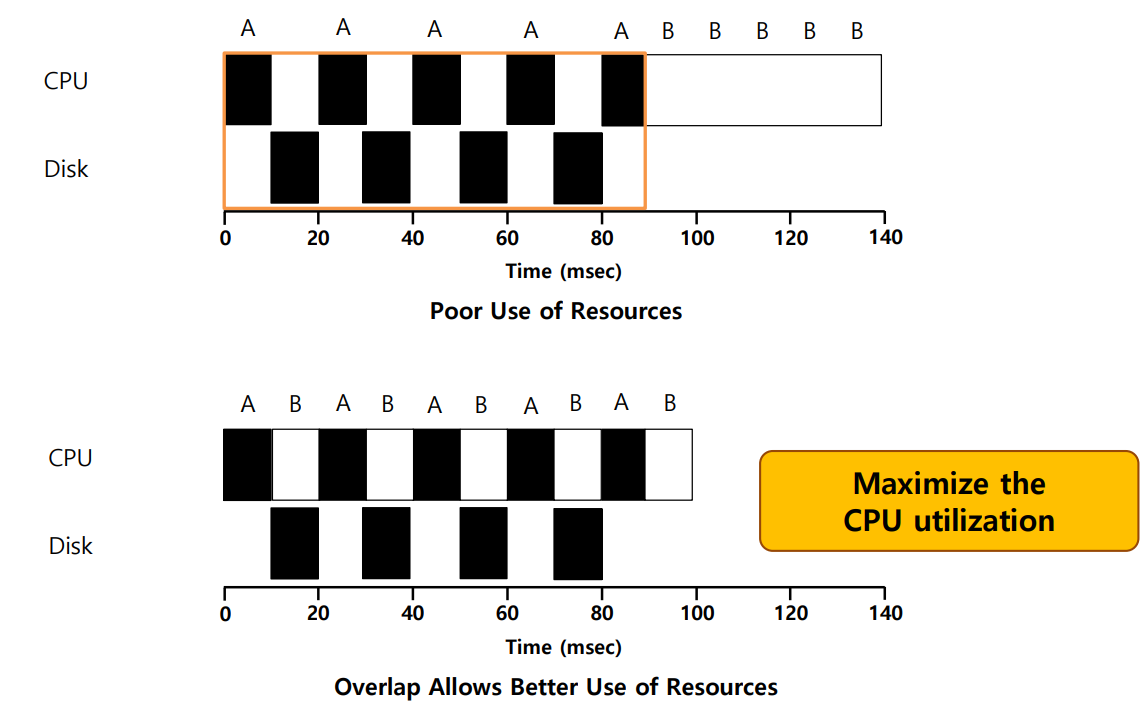
\includegraphics[width=10cm, height=5cm]{Screenshots/Screenshot 2024-10-14 175946.png} % Percorso dell'immagine
    \caption{Gestione dell'I/O} % Didascalia per l'immagine
    \label{fig:immagine} % Etichetta per riferimento
\end{figure}
\subsection{Multi-Level Feedback Queue (MLFQ)}
Con le altre politiche di scheduling abbiamo notato che per migliorare il turnaround time ottenevamo 
un tempo di risposta pessimo mentre per migliorare il tempo di risposta ottenevamo un turnaround 
time più elevato. Quello che tenta di fare il MLFQ è di ottimizzare il turnaround time e minimizzare il 
tempo di risposta, senza sapere a priori il tempo di esecuzione del processo. Questa politica di 
scheduling impara a run-time le caratteristiche dei job da eseguire, in modo tale da prendere delle 
decisioni migliori. MLFQ ha un numero di code distinte, ogni coda ha un livello di priorità. \\
RULE 1: se la $PRIORITA(a) > PRIORITA(b)$ viene eseguito a\\ 
RULE 2: se la $PRIORITA(a) = PRIORITA(b)$ a e b vengono eseguiti in RR\\
\begin{figure}[h]
    \centering
    \begin{minipage}{0.4\textwidth} % Imposta la larghezza della colonna sinistra
        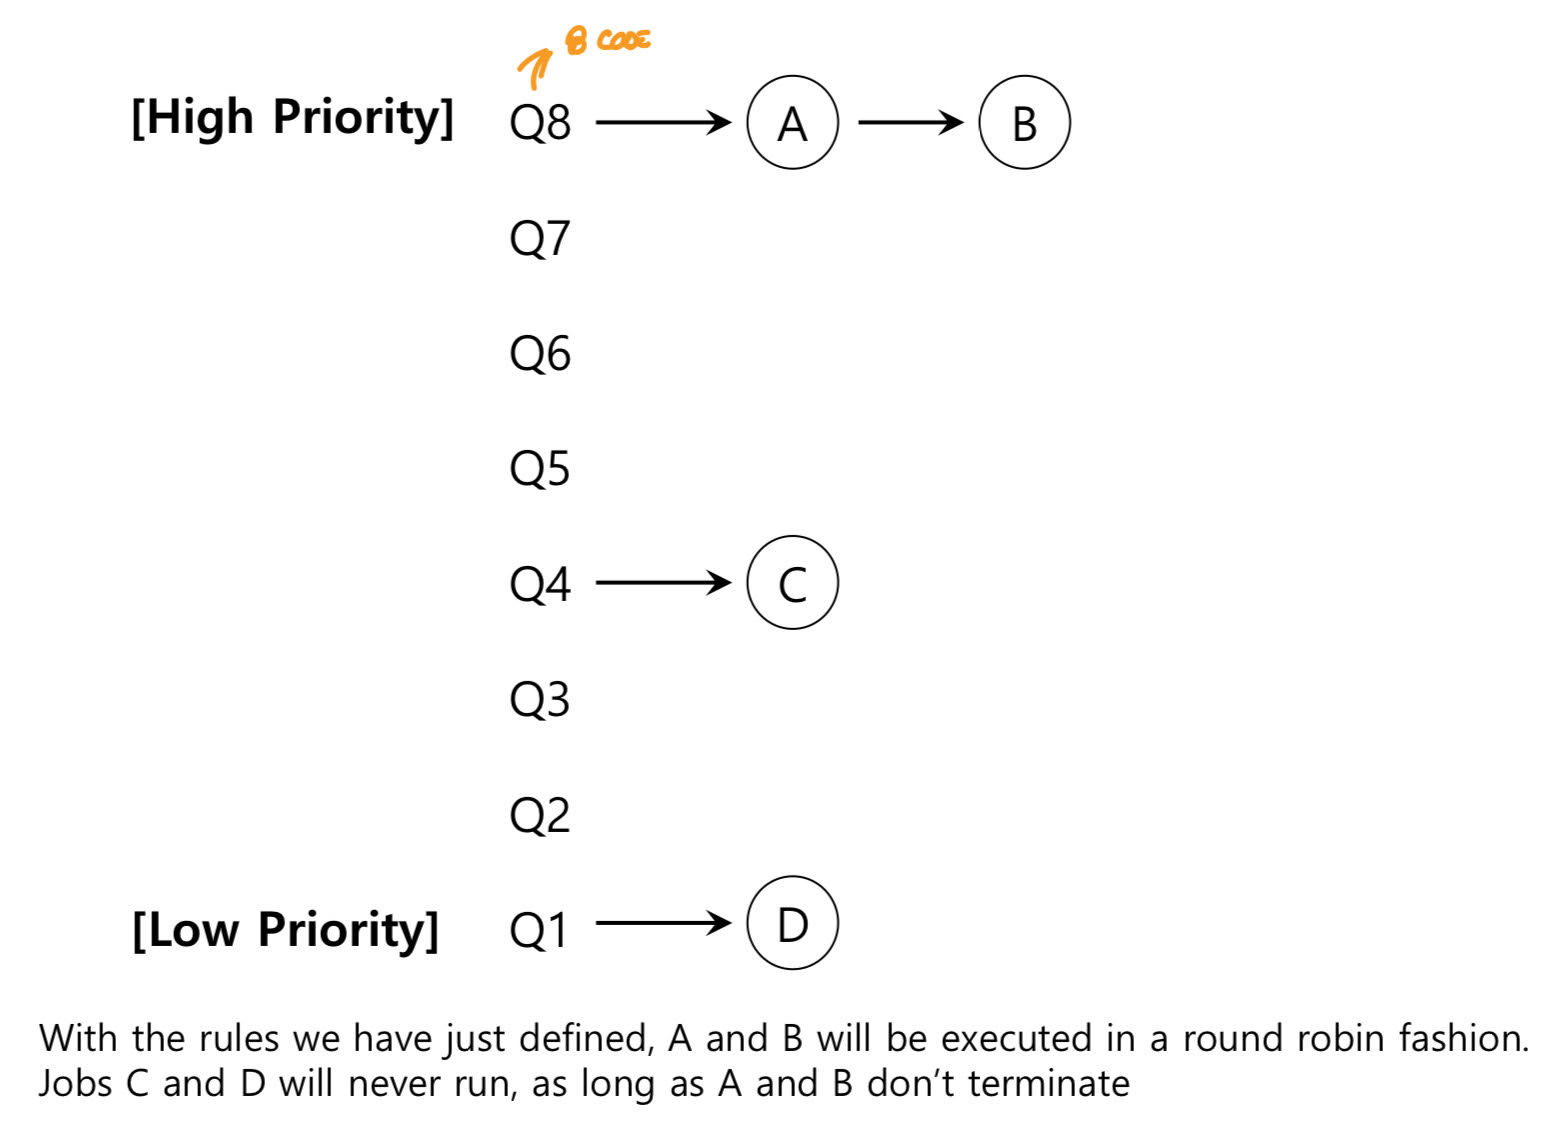
\includegraphics[width=\linewidth]{Screenshots/unnamed (2).jpg}
        \caption{MLFQ e le regole appena definite} % Opzionale
        \label{fig:immagine}
    \end{minipage}%
    \hfill
    \begin{minipage}{0.55\textwidth} % Imposta la larghezza della colonna destra
        A e B vengono eseguiti in Round Robin, C e D non verranno mai eseguiti finchè A e B non terminano
    \end{minipage}
\end{figure}

\vspace{1pt} % Aggiunge uno spazio verticale tra le due sezioni (opzionale)
\noindent %Per togliere lo spazietto fastidioso
MLFQ cambia la priorità di un job osservandone il comportamento:\\
Se un job rilascia spesso la CPU per fare un’operazione di I/O gli lascia la priorità alta dato che probabilmente è un job interattivo e vogliamo che i job interattivi siano reattivi. Se un job utilizza la CPU per un lungo periodo di tempo gli riduce la priorità, questo perché si sta comportando come un job batch (es. avvio un calcolo la sera e la mattina ne vedo il risultato).\\ Aggiungiamo delle regole al cambio di priorità:\\
RULE 3: Quando un job entra nel sistema gli viene attribuita la massima priorità\\
RULE 4a: Quando un job usa un intero quanto di tempo la sua priorità viene ridotta, questo perché potrebbe essere un job batch che richiede la cpu e non esegue operazioni di I/O\\
RULE 4b: Se un job rilascia la CPU prima che finisca il quanto di tempo la sua priorità rimane allo stesso livello, questo perché potrebbe essere un job interattivo\\
Esempio:\\
Il job A ha già avuto modo di dimostrare che non è un job interattivo\\
Il job B è un job interattivo che ha runtime 20ms\\
A è stato eseguito per una certa quantità di tempo, successivamente arriva B al tempo $T=100ms$
\begin{figure}[h]
    \centering
    \begin{minipage}{0.4\textwidth} % Imposta la larghezza della colonna sinistra
        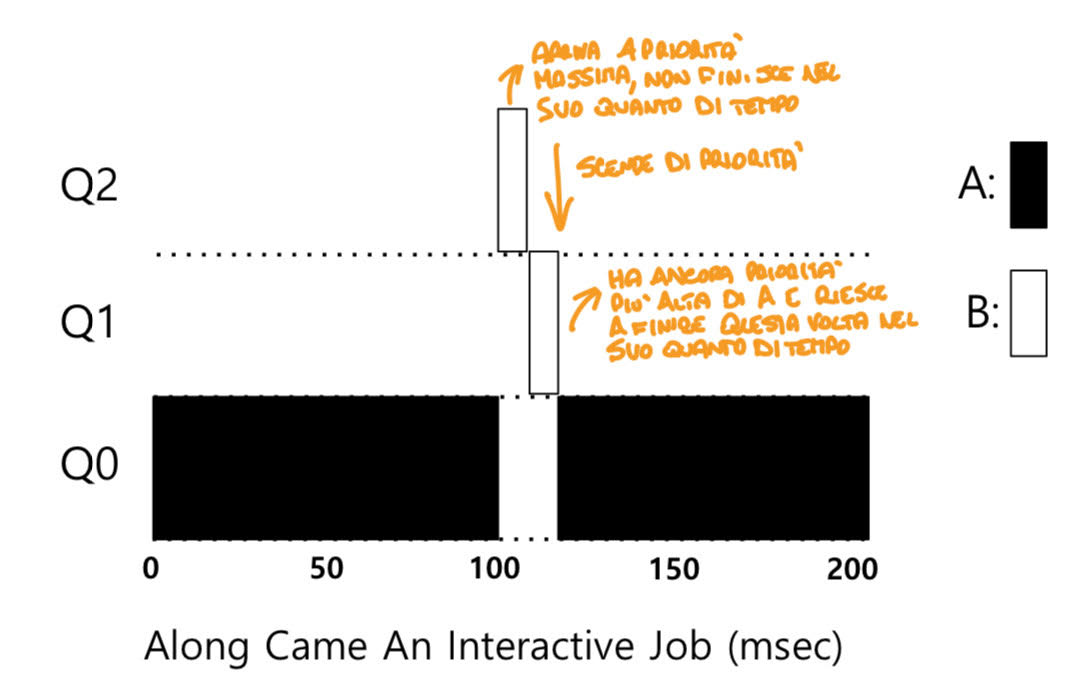
\includegraphics[width=\linewidth]{Screenshots/unnamed (3).jpg}
        \caption{MLFQ con regole 4a e 4b } % Opzionale
        \label{fig:immagine}
    \end{minipage}%
    \hfill
    \begin{minipage}{0.55\textwidth} % Imposta la larghezza della colonna destra
        B arriva a massima priorità e non riesce a finire la sua esecuzione, gli viene scalato un livello di priorità, ha ancora priorità più alta di A e riesce a finire questa volta nel suo quanto di tempo
    \end{minipage}
\end{figure}

\vspace{1pt} % Aggiunge uno spazio verticale tra le due sezioni (opzionale)
\noindent %Per togliere lo spazietto fastidioso
Comparando MLFQ con SJF (Short Job First) SJF doveva sapere a priori la lunghezza di ogni processo, con il set di regole che abbiamo messo MLFQ approssima SJF. La differenza è che MLFQ non gli serve sapere a priori la lunghezza del job, quando arriva un nuovo processo viene messo alla priorità massima, infatti se fosse un processo corto resterebbe alla massima priorità e lavorerebbe come SJF, se invece il processo fosse lungo, quest'ultimo, calerebbe di priorità.
\begin{figure}[h]
    \centering
    \begin{minipage}{0.4\textwidth} % Imposta la larghezza della colonna sinistra
        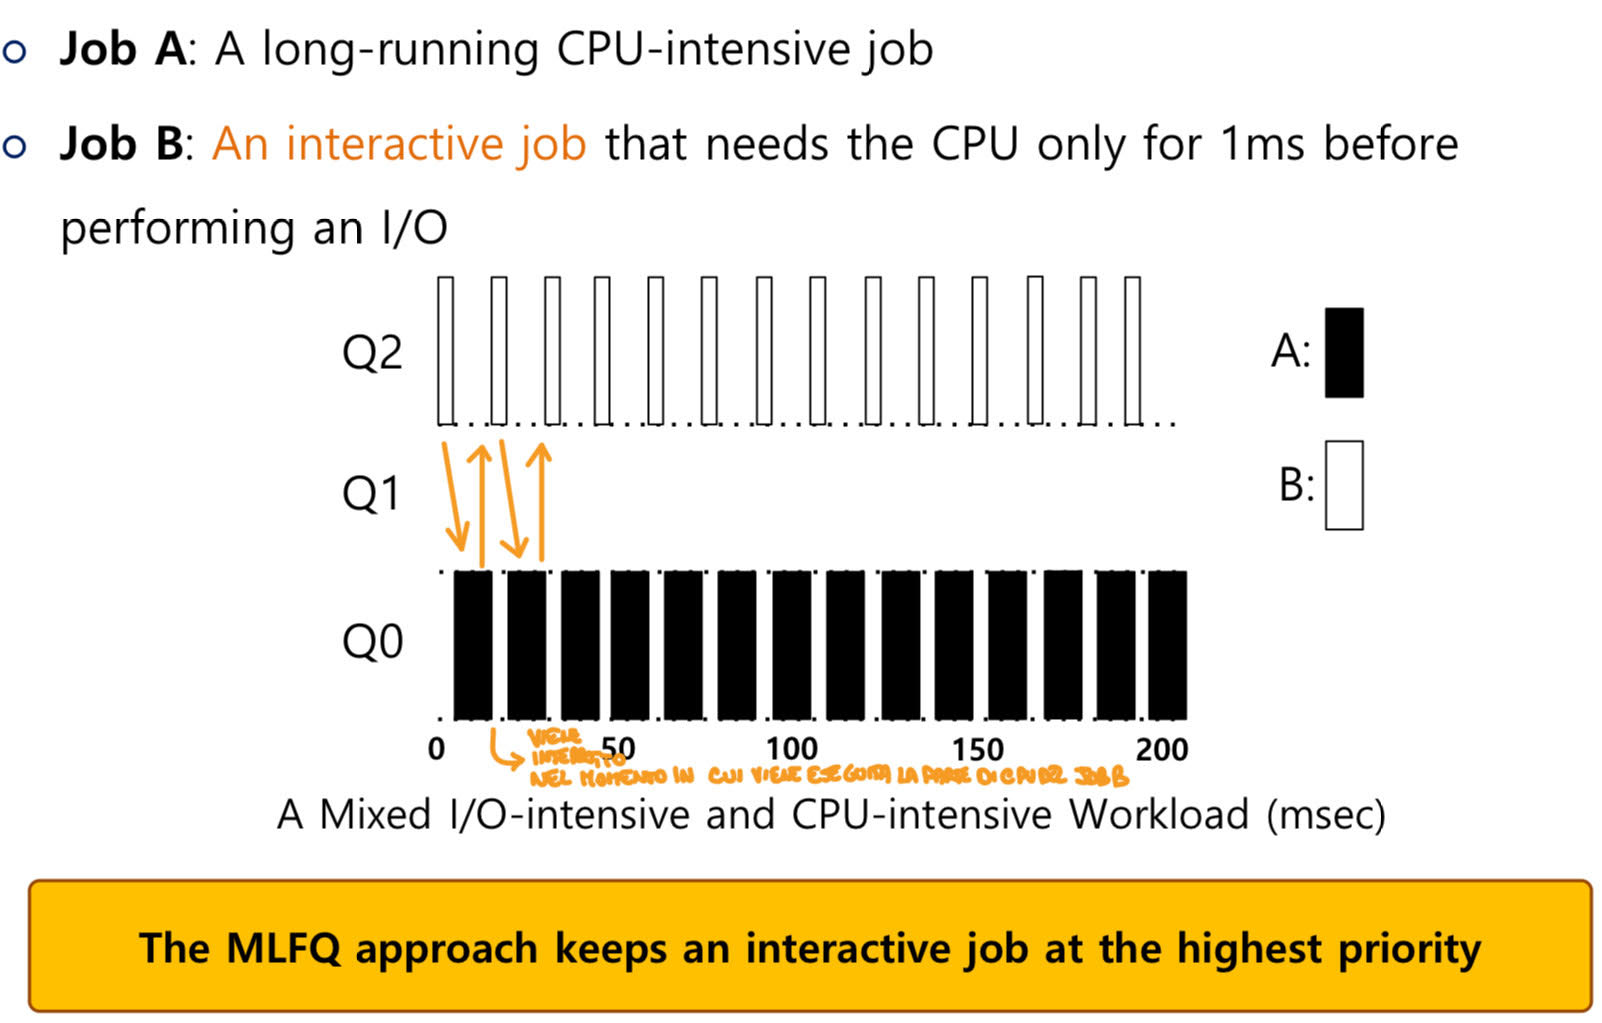
\includegraphics[width=\linewidth]{Screenshots/unnamed (4).jpg}
        \caption{MLFQ con job batch e job interattivo} % Opzionale
        \label{fig:immagine}
    \end{minipage}%
    \hfill
    \begin{minipage}{0.55\textwidth} % Imposta la larghezza della colonna destra
        Quest’esempio ci fa notare delle debolezze:
-Starvation (morire di fame): Se ci fossero troppi job interattivi, i job a priorità più bassa potrebbero andare in starvation.
-Ingannare lo scheduler: Un job malevolo, potrebbe, usare il 99\% del quanto di tempo e successivamente fare una richiesta I/O in modo tale da non perdere di priorità

    \end{minipage}
\end{figure}

\vspace{1pt} % Aggiunge uno spazio verticale tra le due sezioni (opzionale)
\noindent %Per togliere lo spazietto fastidioso
RULE 5 (Priority Boost): Dopo un certo periodo di tempo, sposto tutti i job a priorità massima (“gli do una seconda possibilità”), in poche parole dopo un po' un job batch verrebbe messo a RR con i job interattivi. \\  
RULE 4: (Riscrivo 4a e 4b) Il job passa a un livello di priorità inferiore se viene eseguito per il tempo del quanto di tempo. Es: Ho un job malevolo e ho quanti di tempo da 10ms, utilizza 9ms e poi fa una richiesta di I/O quando verrà poi rieseguito, avrà a disposizione solo 1ms, dopodichè scenderebbe di priorità    \\    
MLFQ solitamente attribuisce ai livelli di priorità più alti quanti di tempo minori e viceversa. L’implementazione Solaris di MLFQ ha 60 code, e incrementa lentamente i quanti di tempo: Livello di priorità massimo: 20ms, Livello di priorità minimo qualche centinaia di ms. Il priority boost viene fatto ogni secondo.                                                         
\subsection{The Linux Completely Fair Scheduling (CFS)}
È la politica di scheduling che troviamo sulle macchine di adesso. Le sue principali caratteristiche sono: quanti di tempo variabili, supporta la priorità, controlla la priorità secondo un parametro di “gentilezza” (quanto il nostro processo debba essere gentile con gli altri processi) , utilizza delle strutture dati che sono più efficienti per ricerca, inserzione e cancellazione di un processo. I parametri base sono:\\
\paragraph{Virtual Runtime (Vruntime)}: Denota per quanto tempo un processo è stato eseguito, ovvero la quantità in ms di cpu utilizzata dal processo. Incrementa proporzionalmente durante l’esecuzione di un job. Il CFS prenderà il processo avente runtime più basso possibile.
\paragraph{Sched\_Latency}: è il parametro che definisce la dimensione della finestra temporale da dividere in quanti di tempo (definendo questo parametro guadagnamo in termini di tempo di risposta), un valore tipico è di 48 ms. Il quanto di tempo di un processo $= \frac{sched\_latency}{numero di processi}$.
\begin{figure}[H] % Usa 'H' per forzare la posizione qui
    \centering % Centra l'immagine
    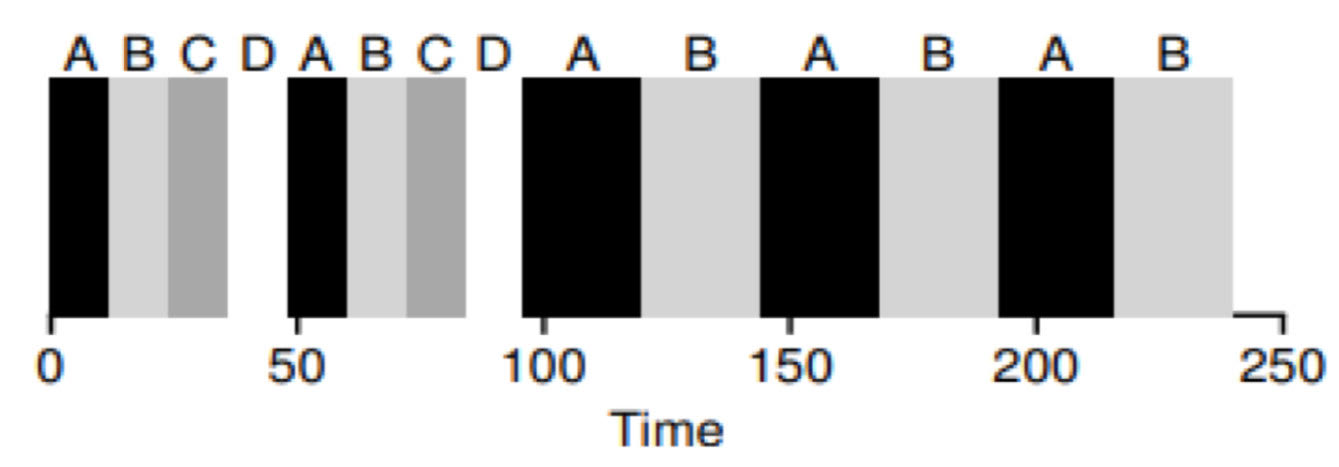
\includegraphics[width=10cm, height=4cm]{Screenshots/unnamed (5).jpg} % Percorso dell'immagine
    \caption{Esempio per capire il concetto di var} % Didascalia per l'immagine
    \label{fig:immagine} % Etichetta per riferimento
\end{figure}
\noindent %Per togliere lo spazietto fastidioso
Ora c’è bisogno di fare delle precisazioni: il quanto di tempo minimo è di 6ms, infatti se riducessimo troppo il tempo dei quanti di tempo il SO impiegherebbe più tempo a fare il context switching che a eseguire i processi stessi. Il parametro di gentilezza va da -20 a +1 e viene tradotto in pesi numerici.
\begin{figure}[H] % Usa 'H' per forzare la posizione qui
    \centering % Centra l'immagine
    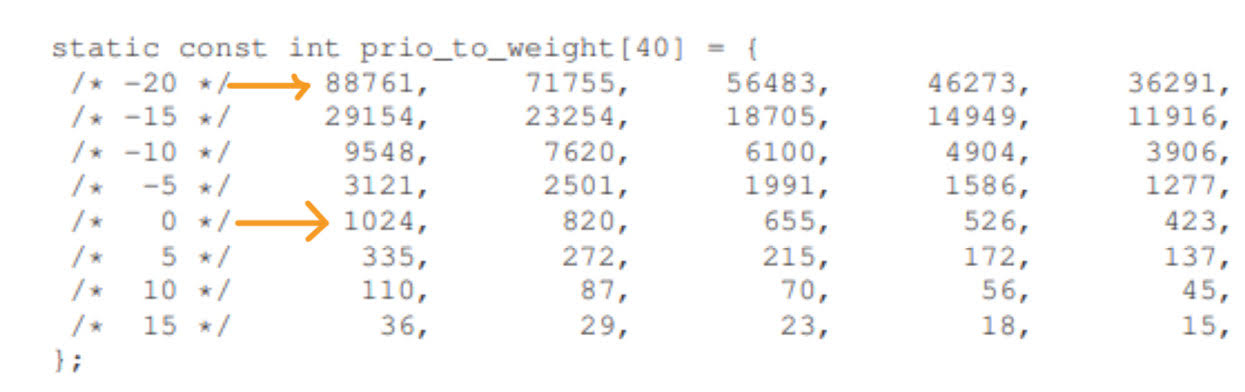
\includegraphics[width=13cm, height=4cm]{Screenshots/unnamed (6).jpg} % Percorso dell'immagine
    \caption{Tabella dei pesi} % Didascalia per l'immagine
    \label{fig:immagine} % Etichetta per riferimento
\end{figure}
\vspace{10pt} % Regola questo valore se necessario
\begin{figure}[H] 
    \centering
    \vspace{-10pt} % Riduce lo spazio sopra l'immagine
    \begin{minipage}{0.4\textwidth} % Colonna per le immagini
        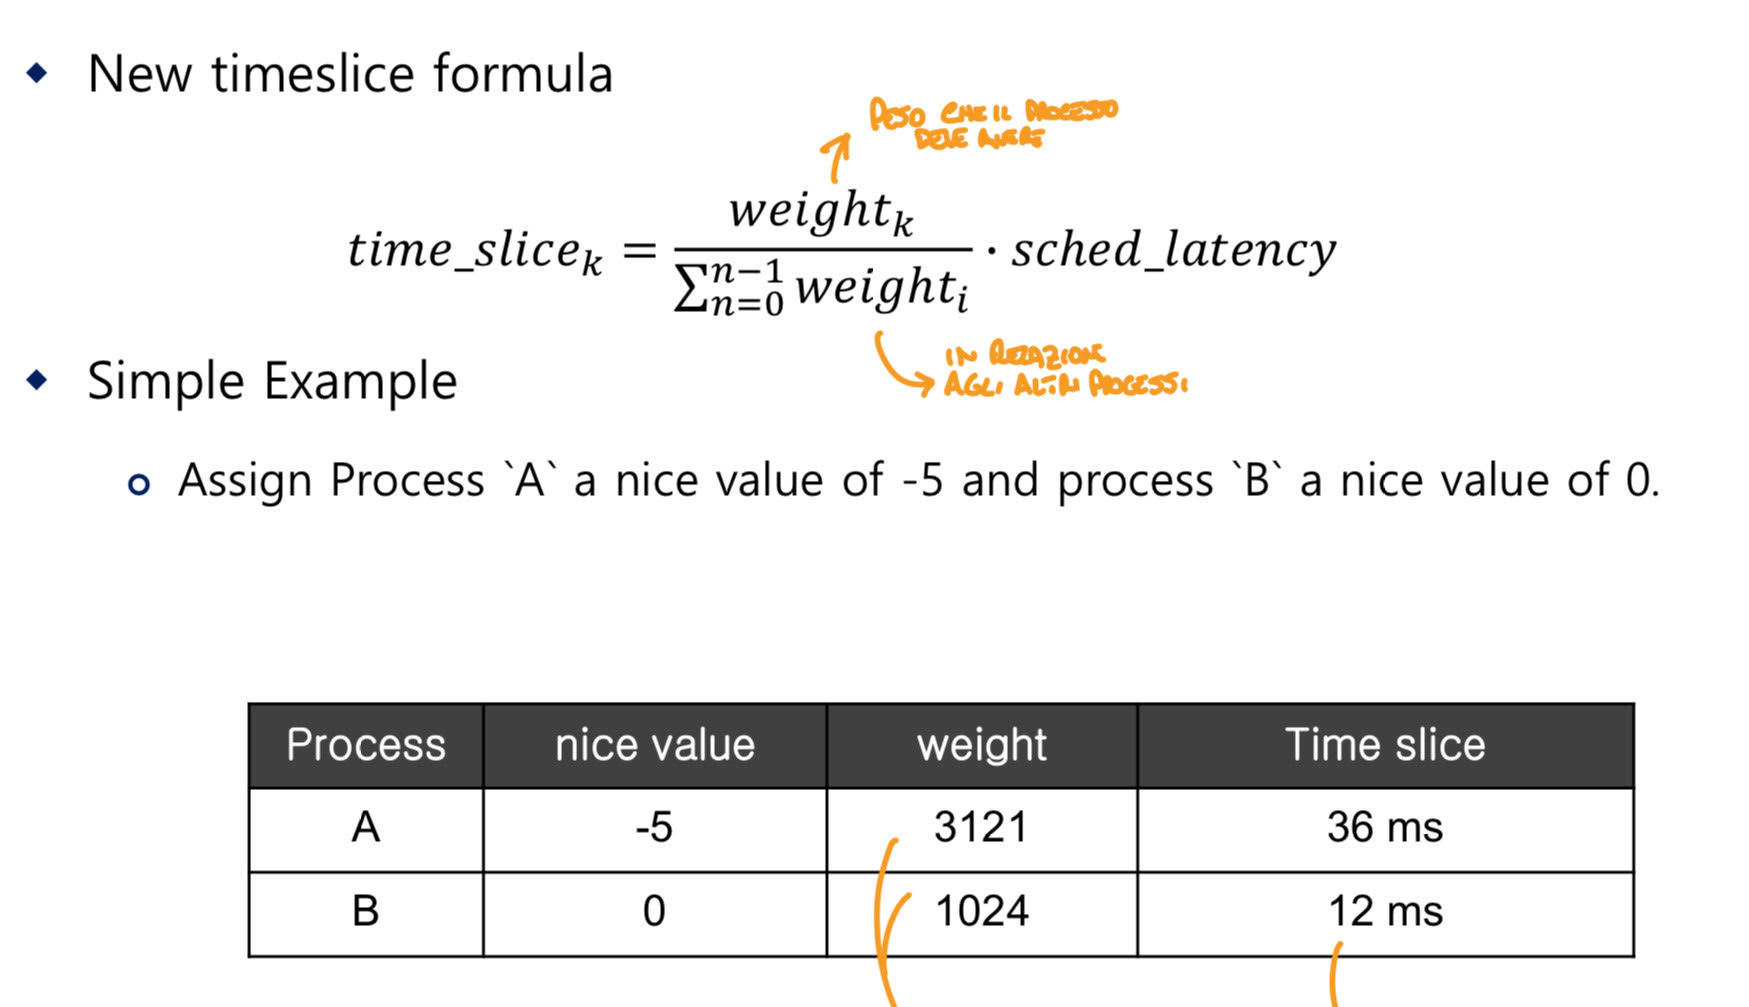
\includegraphics[width=\linewidth]{Screenshots/unnamed (7).jpg} % Prima immagine
        \vspace{10pt} % Spazio verticale tra le immagini
        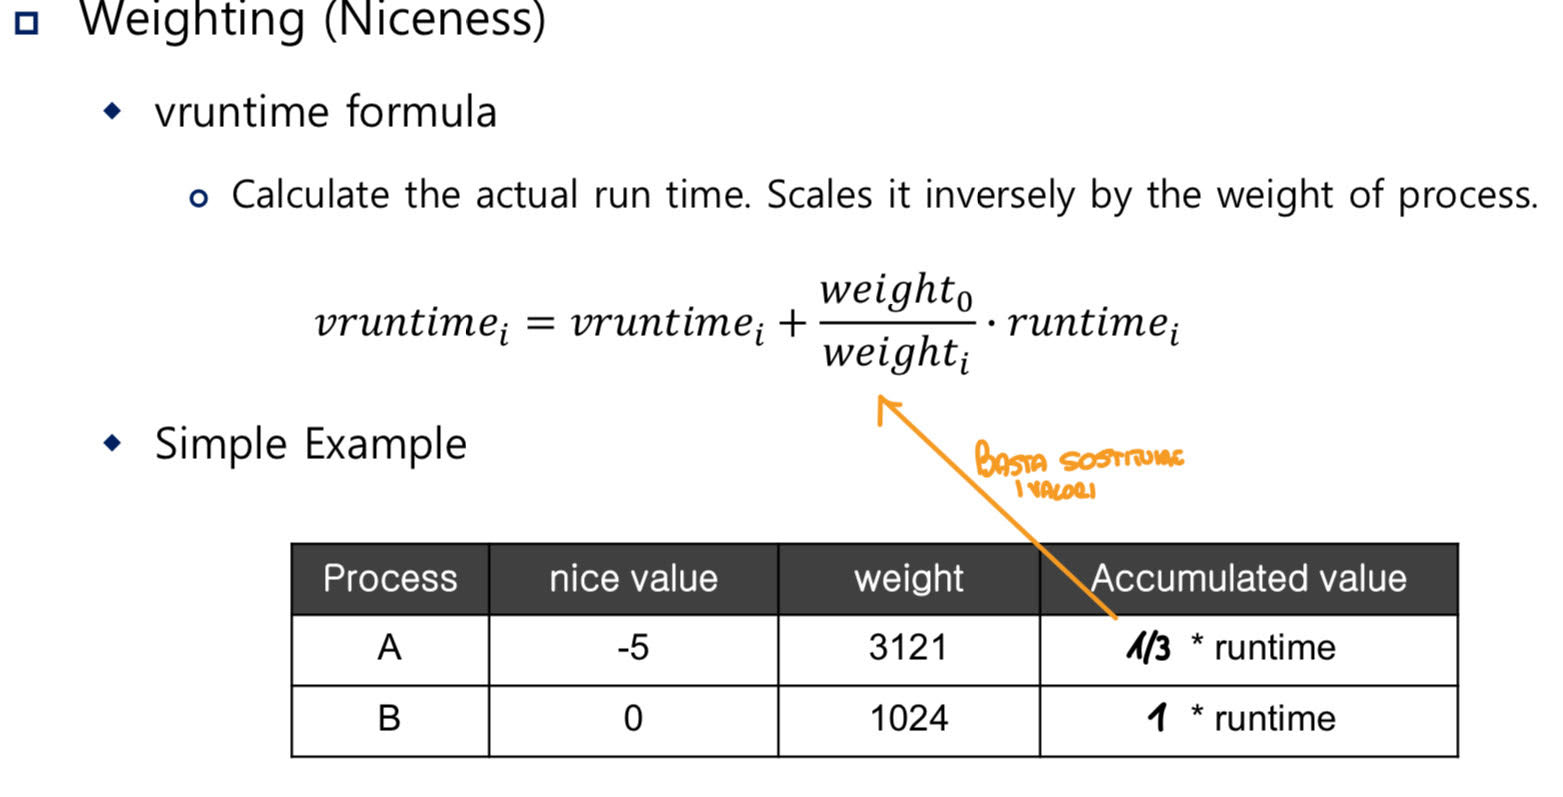
\includegraphics[width=\linewidth]{Screenshots/unnamed (8).jpg} % Seconda immagine
    \end{minipage}%
    \hfill
    \begin{minipage}{0.55\textwidth} % Colonna per il testo
        \textbf{} \noindent Questa è la formula per il quanto di tempo, ovvero $\frac{PesoDelProcesso}{SommaDeiPesiDeiProcessi} \ast sched\_latency$. In questo esempio il processo B verrà preferito dato che B avrà, dopo la prima esecuzione, Vruntime più basso e quindi B raggiungerà A. Per ovviare a questo viene aggiustato il calcolo del Vruntime che sale inversamente al peso del processo.
        
        \vspace{20pt} % Spazio verticale tra i blocchi di testo
        
        \textbf{} Una struttura basata su questo tipo di coda, sono gli alberi rosso-neri. L’ultima osservazione da fare è chiederci cosa succede in caso un processo voglia fare un’operazione di I/O. Innanzitutto bisogna evitare che gli altri processi aventi Vruntime basso monopolizzino la cpu, infatti quello che viene fatto è mettere al minimo il vruntime di tutti i processi.
    \end{minipage}
\end{figure}
\section{Process API/Chiamate di sistema}
\subsection{Introduzione alle chiamate di sistema}
\subsection*{Alcuni cenni prima dell'inizio}
Per \textbf{creare un file.c} bisogna eseguire il comando \textbf{nano hello.c}. Per \textbf{salvare} bisogna premere \textbf{ctrl + o + invio}. Per \textbf{chiudere} il file che abbiamo appena aperto \textbf{ctrl + x}. Per \textbf{compilare} il file eseguiamo il comando \textbf{gcc -o nome\_da\_dare\_all\_eseguibile file.c}. Per \textbf{eseguire} il file aggiungiamo \textbf{./} davanti al nome dell eseguibile. Di notevole importanza il comando \textbf{Man} che apre letteralmente il manuale di una chiamata di sistema.
\subsection{La chiamata di sistema Fork()}
La chiamata di sistema Fork(), fa un salto nel kernel, infatti sdoppia il processo che ha effettuato la chiamata di sistema. Il nuovo processo avrà la sua personale copia dello spazio degli indirizzi, dei registri e di PC. Avremo due processi identici, il quale, quello che ha chiamato la fork lo chiameremo processo padre e l'altro lo chiameremo processo figlio.
\begin{lstlisting}[language=C, frame=single, numbers=left, caption=p1.c]
#include <stdio.h>
#include <stdlib.h>
#include <unistd.h>
int main(int argc, char *argv[]){
printf("hello world (pid:%d)\n", (int) getpid());
int rc = fork();
if (rc < 0) { // fork failed; exit
fprintf(stderr, "fork failed\n");
exit(1);
} else if (rc == 0) { // child (new process)
printf("hello, I am child (pid:%d)\n", (int) getpid());
} else { // parent goes down this path (main)
printf("hello, I am parent of %d (pid:%d)\n",
rc, (int) getpid());
}
return 0;}
\end{lstlisting}
\noindent
Il processo che è stato creato dalla chiamata di sistema, non inizierà dalla prima istruzione del main ma dopo la fork. Sostanzialmente nell'esecuzione del programma quello che ci aspettiamo è che i processi genereranno dei valori diversi all'interno della variabile rc e in particolare che il processo figlio imbocchi il ramo con $rc=0$. Se qualcosa fosse andato storto la fork avrebbe restituito un valore $<0$.
\subsection{La chiamata di sistema Wait()}
La chiamata di sistema Wait() sospende l'esecuzione del processo chiamante fino a quando uno dei suoi figli termina l'esecuzione.
\begin{lstlisting}[language=C, frame=single, numbers=left, caption=p2.c]
#include <stdio.h>
#include <stdlib.h>
#include <unistd.h>
#include <sys/wait.h>
int main(int argc, char *argv[]){
printf("hello world (pid:%d)\n", (int) getpid());
int rc = fork();
if (rc < 0) { // fork failed; exit
fprintf(stderr, "fork failed\n");
exit(1);
} else if (rc == 0) { // child (new process)
printf("hello, I am child (pid:%d)\n", (int) getpid());
} else { // parent goes down this path (main)
int wc = wait(NULL);
printf("hello, I am parent of %d (wc:%d) (pid:%d)\n",
rc, wc, (int) getpid());
}
return 0;
}
\end{lstlisting}
\noindent
Passiamo come parametro alla chiamata di sistema Wait() un puntatore nullable e ci aspettiamo che ci restituisca il PID del processo che ha cambiato il suo stato per primo.
\subsection{Il programma analizzato in aula}
Abbiamo creato un programma in aula che ci consenta di scrivere all'interno di un file
\begin{lstlisting}[language=C, frame=single, numbers=left, caption=scrittura\_file.c]
#include <stdio.h> 
#include <fcntl.h> 
#include <string.h> 
#include <unistd.h> 
int main(){ 
 
       char messaggio[]="ciao"; 
       int fd=open("pippo.txt", O_CREAT | O_TRUNC | O_WDONLY, S_IRWXU); 
       write(fd, messaggio, strlen(messaggio)); 
       close(fd); 
}
\end{lstlisting}
\noindent
In particolare: \textbf{O\_CREAT} crea il file in caso non venga trovato, \textbf{O\_TRUNC} se il file già esiste sarà troncato a 0, \textbf{O\_WRONLY} indica che siamo interessati soltanto a scrivere il file e successivamente attribuisco al file i permessi \textbf{S\_IRWXU} che indicano che il possessore del file può leggerlo, scriverlo e eseguirlo.\\\\
Se invece fossimo interessati a \textbf{leggere} il contenuto di pippo.txt dovremmo utilizzare la chiamata di sistema \textbf{read()} questa prende come primo parametro un file descriptor e come secondo un buffer che serve a immettere l'informazione che stiamo leggendo nella memoria.
\begin{lstlisting}[language=C, frame=single, numbers=left, caption=lettura\_file.c]
#include <stdio.h> 
#include <fcntl.h> 
#include <unistd.h> 
int main(){ 
 
        int fd= open("pippo.txt", O_RDONLY, S_IRWXU); 
        int buffer=0; 
        read(fd, &buffer, sizeof(int)); 
        printf("Buffer: %d\n", buffer); 
        close(fd); 
} 
\end{lstlisting}
\subsection{La chiamata di sistema Exec()}
La chiamata di sistema Exec() ci consente di eseguire altre applicazioni dal programma che stiamo utilizzando. Questa chiamata ha vari utilizzi i quali hanno diversa sintassi, in particolare abbiamo visto la execv che ha come primo parametro una stringa che fa riferimento al percorso dell'eseguibile che vogliamo andare a eseguire. La stringa che andiamo a passare come parametro sarà composta in questo modo: la posizione 0 fa riferimento al percorso dell'eseguibile e sarà seguita dagli argomenti che vogliamo passare all'eseguibile, l'ultimo elemento deve essere necessariamente NULL.
\begin{lstlisting}[language=C, frame=single, numbers=left, caption=Chiamata di sistema Exec()]
#include <stdio.h> 
#include <fcntl.h> 
#include <unistd.h> 
#include <string.h>
int main(){ 
 
        int fd= open("pippo.txt", O_RDONLY, S_IRWXU); 
        int buffer=0; 
        read(fd, &buffer, sizeof(int)); 
        printf("Buffer: %d\n", buffer); 
        close(fd); 
        char *myarg[2];
        myarg[0]=strdup("ls"); //vado a mettere all interno di myarg[0]
                               //un puntatore a qualcosa che sta dentro
                               //l heap
        myarg[1]=NULL;
        execv(myarg[0], myarg);
        printf("CIAO\n"); //questo non viene letto perche l'esecuzione
                          //si ferma a execv
} 
\end{lstlisting}
\section{Spazio degli indirizzi}
\subsection{Introduzione allo spazio degli indirizzi}
Abbiamo visto come la CPU possa essere virtualizzata in modo tale da ospitare più processi in esecuzione e vorremmo ottenere lo stesso effetto anche per la memoria. Parliamo di \textbf{virtualizzazione della memoria}, il sistema operativo virtualizza la memoria e fornisce uno spazio di memoria illusorio a ogni processo. Questo processo rende la memoria più efficiente in termini di spazio e tempo e garantisce l'isolamento per i processi e il sistema operativo. Infatti, non vogliamo che un processo anche se benevolo, cambi qualcosa, questo perchè anche il minimo cambiamento potrebbe far crashare il sistema.
\subsection{Gestione della memoria nei primi sistemi}
\begin{figure}[h]
    \centering
    \begin{minipage}{0.4\textwidth} % Imposta la larghezza della colonna sinistra
        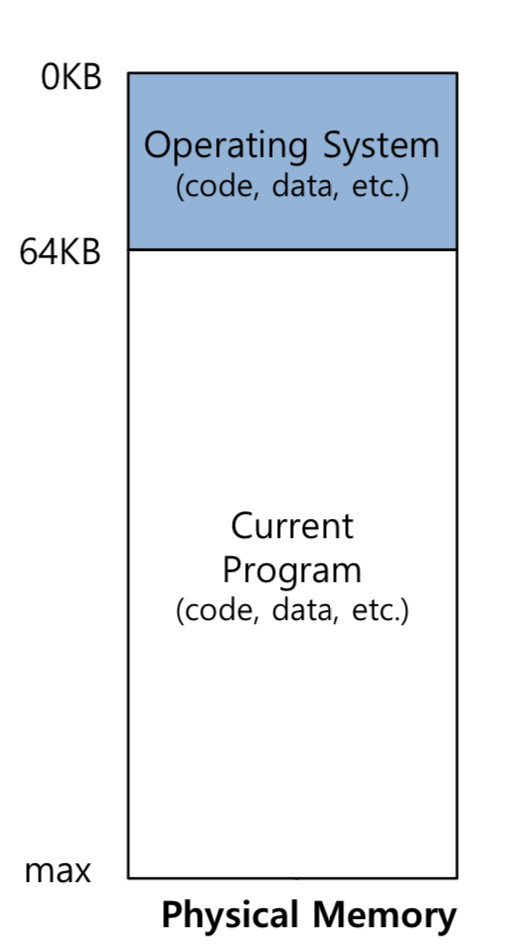
\includegraphics[width=4cm, height=5cm]{IMG_0790.jpeg}
        \caption{Gestione della memoria nei primi sistemi} % Opzionale
        \label{fig:immagine}
    \end{minipage}%
    \hfill
    \begin{minipage}{0.55\textwidth} % Imposta la larghezza della colonna destra
       Veniva caricato un solo processo in memoria, questo però aveva uno scarso utilizzo e efficienza. Come pro aveva delle prestazioni ineguagliabili per l'accesso in memoria

    \end{minipage}
\end{figure}


\noindent %Per togliere lo spazietto fastidioso
\subsection{Gestione della memoria con multiprogrammazione e Time Sharing}
\begin{figure}[h]
    \centering
    \begin{minipage}{0.4\textwidth} % Imposta la larghezza della colonna sinistra
        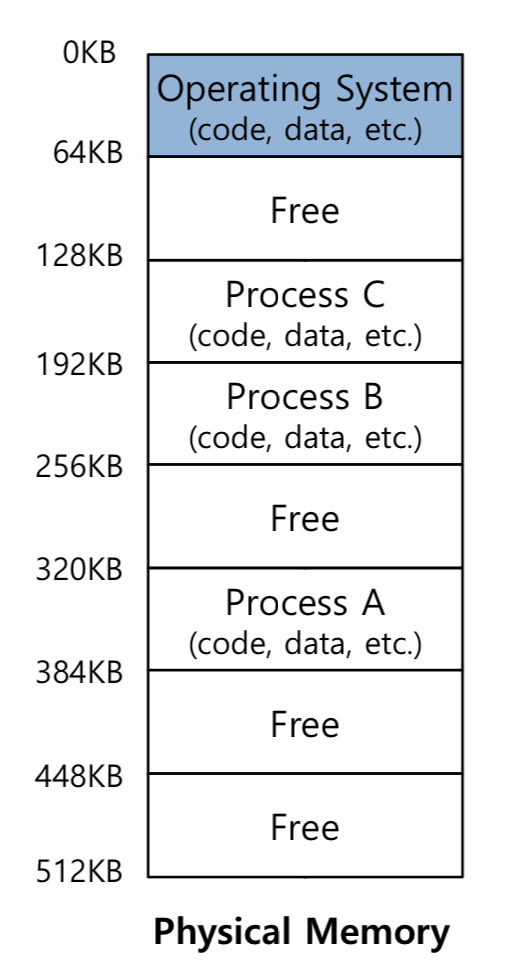
\includegraphics[width=4cm, height=5cm]{IMG_0791.jpeg}
        \caption{Gestione della memoria con multiprogrammazione e Time Sharing} % Opzionale
        \label{fig:immagine}
    \end{minipage}%
    \hfill
    \begin{minipage}{0.55\textwidth} % Imposta la larghezza della colonna destra
       Vengono caricati più processi in memoria, si passa da un processo all'altro che viene eseguito per un piccolo quanto di tempo, questo imcrementa l'utilizzo e l'efficienza. Il suo contro è che vi si possono causare degli errati accessi in memoria da parte dei processi

    \end{minipage}
\end{figure}

\vspace{100pt} % Aggiunge uno spazio verticale tra le due sezioni (opzionale)
\noindent %Per togliere lo spazietto fastidioso
\subsection{Gestione della memoria con lo spazio degli indirizzi}
\begin{figure}[h]
    \centering
    \begin{minipage}{0.4\textwidth} % Imposta la larghezza della colonna sinistra
        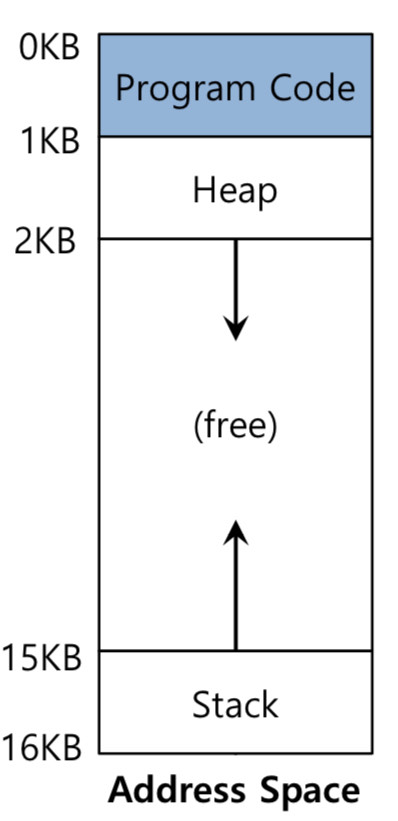
\includegraphics[width=4cm, height=6cm]{IMG_0792.jpeg}
        \caption{Gestione della memoria con lo spazio degli indirizzi} % Opzionale
        \label{fig:immagine}
    \end{minipage}%
    \hfill
    \begin{minipage}{0.55\textwidth} % Imposta la larghezza della colonna destra
       Come abbiamo detto il sistema operativo astrae la memoria fisica. Lo spazio degli indirizzi contiene tutto riguardo il processo in esecuzione, che consiste in codice del programma, heap, stack...\\
       Ogni processo avendo il proprio spazio degli indirizzi avrà l'illusione di avere uno spazio privato sulla memoria, invece sarà compito del sistema operativo abbinare gli indirizzi virtuali agli indirizzi fisici\\
       \textbf{Program Code}: è la parte dove vivono le istruzioni\\
       \textbf{Heap}: è dove viene allocata dinamicamente la memoria (malloc (C), new (programmazione orientata agli oggetti)\\
       \textbf{Stack}: dove vengono immagazzinati i valori e gli indirizzi di ritorno, contiene variabili locali e argomenti.

    \end{minipage}
\end{figure}

\vspace{1pt} % Aggiunge uno spazio verticale tra le due sezioni (opzionale)
\noindent %Per togliere lo spazietto fastidioso
Un'altro esempio che ci permette di comprendere lo spazio degli indirizzi è questo codice, infatti lanciandolo diverse volte sembrerà che il programma utilizzi sempre gli stessi indirizzi, questo perchè sono virtuali. 
\begin{lstlisting}[language=C, frame=single, numbers=left, caption=Spazio degli indirizzi]
#include <stdio.h>
#include <stdlib.h>
int main(int argc, char *argv[]){
    printf("location of code : %p\n", (void *) main);
    printf("location of heap : %p\n", (void *) malloc(1));
    int x = 3;
    printf("location of stack : %p\n", (void *) &x);
    return x;
}

\end{lstlisting}
\section{Traduzione degli indirizzi}
\subsection{Introduzione alla traduzione degli indirizzi}
Come per la vitualizzazione della CPU, vogliamo ottenere un meccanismo efficiente e controllabile per la virtualizzazione della memoria, anche qui sarà necessario il supporto hardware. Questo supporto consiste nella trasformazione da indirizzo virtuale a indirizzo fisico. 
\subsection{Assunzioni per iniziare l'analisi della traduzione degli indirizzi}
Lo spazio degli indirizzi di un processo deve essere collocato contiguamente nella memoria fisica.\\\\
La dimensione dello spazio degli indirizzi è più piccola della dimensione della memoria fisica\\\\
Ogni spazio degli indirizzi ha la stessa dimensione\\\\
\subsection{Applicazione che accede alla memoria}
In codice C: viene caricato il valore dalla memoria, viene incrementato di tre e memorizzato nella memoria
\begin{lstlisting}[language=C, frame=single, numbers=left]
void func() {
    int x;
    ...
    x= x+3; 
}
\end{lstlisting}
\noindent
In Assembly: viene caricato il valore dell'indirizzo dentro il registro eax, viene aggiunto 3 al registro eax, viene caricato il valore dentro eax nella memoria
\begin{lstlisting}[language=C, frame=single, numbers=left]
128 : movl 0x0(%ebx), %eax ; load 0+ebx into eax
132 : addl $0x03, %eax ; add 3 to eax register
136 : movl %eax, 0x0(%ebx) ; store eax back to mem
\end{lstlisting}

\begin{figure}[h]
    \centering
    \begin{minipage}{0.4\textwidth} % Imposta la larghezza della colonna sinistra
        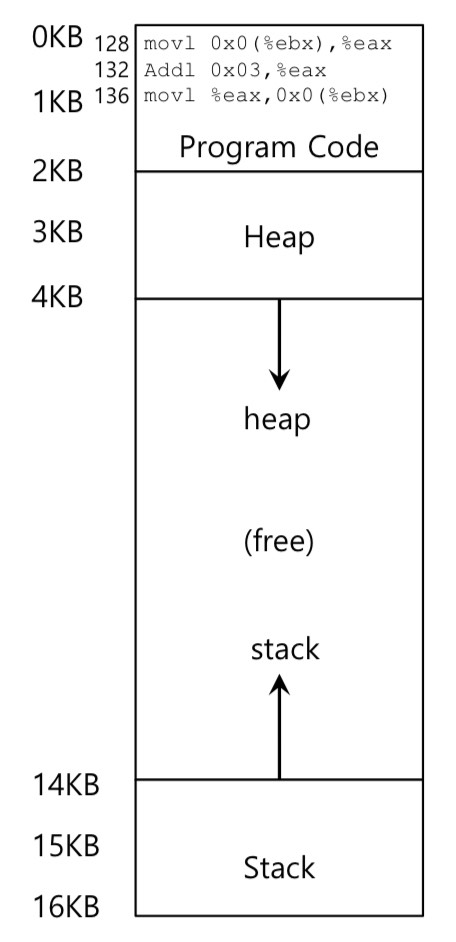
\includegraphics[width=4cm, height=8cm]{IMG_0793.jpeg}
        \caption{Applicazione che accede alla memoria} % Opzionale
        \label{fig:immagine}
    \end{minipage}%
    \hfill
    \begin{minipage}{0.55\textwidth} % Imposta la larghezza della colonna destra
       Recupera (Fetch) l'istruzione all'indirizzo 128 \\\\
       Esegue l'istruzione (carica dall'indirizzo 15KB)\\\\
       Recupera l'istruzione all'indirizzo 132\\\\
       Esegue l'istruzione\\\\
       Recupera l'istruzione all'indirizzo 136\\\\
       Esegue l'istruzione (Carica all'indirizzo 15KB)\\\\
       

    \end{minipage}
\end{figure}

\vspace{150pt} % Aggiunge uno spazio verticale tra le due sezioni (opzionale)
\noindent %Per togliere lo spazietto fastidioso
\subsection{Registri Base e Bound}
Nel registro \textbf{Base} c'è l'indirizzo iniziale della memoria fisica, nel registro \textbf{Bound} c'è la dimensione dello spazio degli indirizzi che sto tenendo in considerazione. Questi due sono due "pezzi" hardware fisici.
\begin{figure}[H] % Usa 'H' per forzare la posizione qui
    \centering % Centra l'immagine
    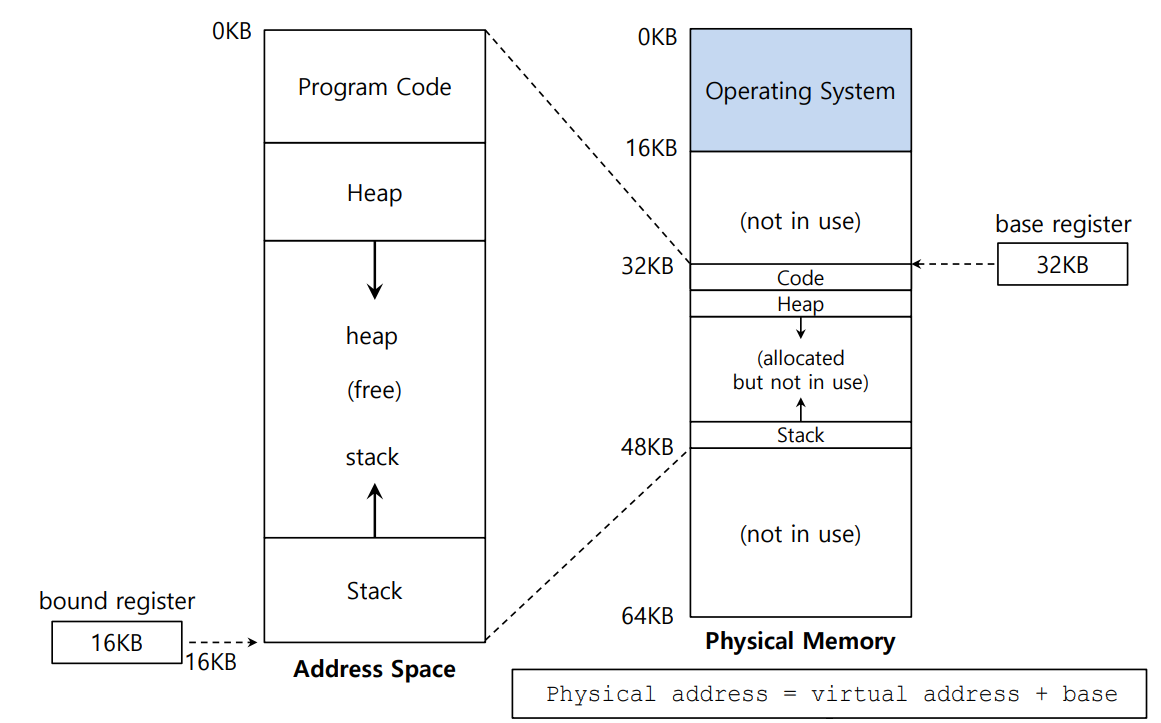
\includegraphics[width=13cm, height=6cm]{immagine_2024-11-01_151046637.png} % Percorso dell'immagine
    \caption{Registri Base e Bound} % Didascalia per l'immagine
    \label{fig:immagine} % Etichetta per riferimento
\end{figure}
\noindent
Se consideriamo solamente il registro Base ci sarebbe un problema, ovvero non vogliamo che qualcuno acceda ad un determinato indirizzo solamente perchè conosce questa formuletta. A tal proposito viene aggiunto il registro Bound infatti grazie ad esso controllo se la richiesta di traduzione dell'indirizzo non sia più grande della dimensione dello spazio degli indirizzi allocato per il processo.
\begin{figure}[h]
    \centering
    \begin{minipage}{0.4\textwidth} % Imposta la larghezza della colonna sinistra
        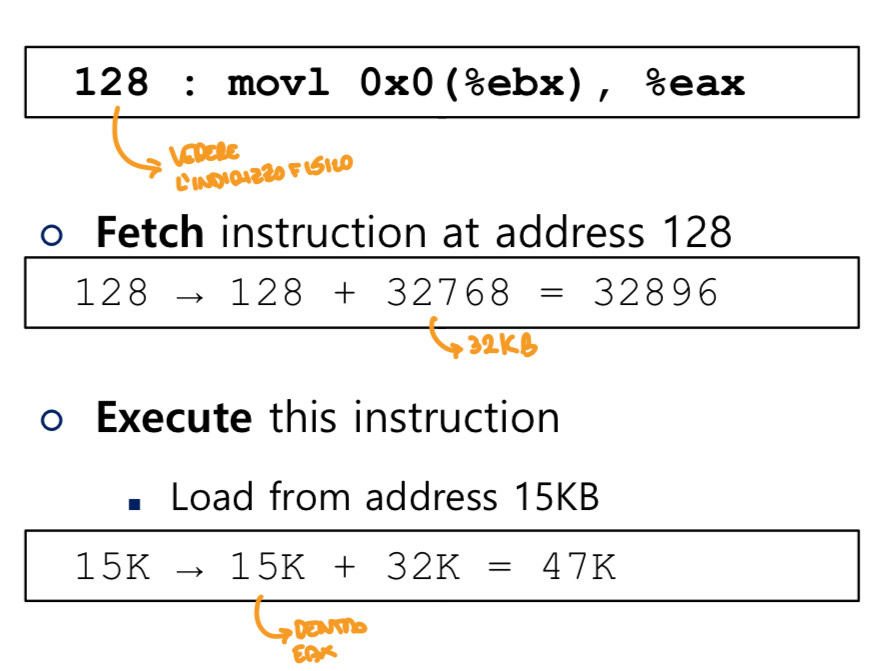
\includegraphics[width=8cm, height=6cm]{IMG_0794.jpeg}
        \label{fig:immagine}
    \end{minipage}%
    \hfill
    \begin{minipage}{0.55\textwidth} % Imposta la larghezza della colonna destra
       Ora capiamo meglio l'esempio di prima:\\\\
       Recupera (Fetch) l'istruzione all'indirizzo 128 (traduzione)\\\\
       Esegue l'istruzione (carica dall'indirizzo 15KB)\\\\

    \end{minipage}
\end{figure}
\noindent %Per togliere lo spazietto fastidioso
\paragraph{Completamento da parte del sistema operativo}
Il supporto che ci fornisce l'hardware non è male, ma va completato con l'implementazione con il sistema operativo. Il sistema operativo deve prendere dei provvedimenti per implementare l'approccio base-and-bound. Ci sono tra punti di giunzione critici: quando un processo inizia l'esecuzione, bisogna trovare uno spazio degli indirizzi sufficientemente grande nella memoria fisica, quando un processo termina, va reclamata la memoria e infine quando si verifica il context switch, in cui bisogna salvare e caricare i valori dei registri base e bound.
\subsection{Primo problema: quando un processo inizia l'esecuzione}
Il sistema operativo deve trovare uno spazio per lo spazio degli indirizzi: viene quindi istanziata una free list, ovvero, una lista di range della memoria fisica che non sono in uso. Solitamente è da slot di 16KB
\subsection{Secondo problema: quando un processo viene terminato}
Il sistema operativo rimette nella free list la memoria.
\begin{figure}[H] % Usa 'H' per forzare la posizione qui
    \centering % Centra l'immagine
    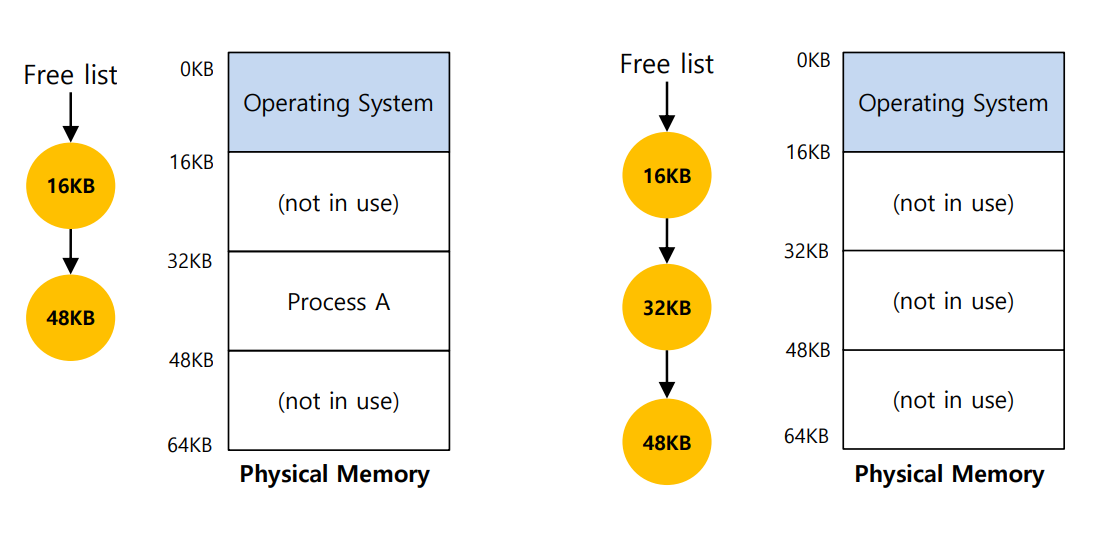
\includegraphics[width=13cm, height=6cm]{immagine_2024-11-01_160045779.png} % Percorso dell'immagine
    \caption{} % Didascalia per l'immagine
    \label{fig:immagine} % Etichetta per riferimento
\end{figure}
\noindent
\subsection{Terzo problema: quando si verifica il context switch}
Il sistema operativo salva i valori dei registri Base e Bound
\begin{figure}[H] % Usa 'H' per forzare la posizione qui
    \centering % Centra l'immagine
    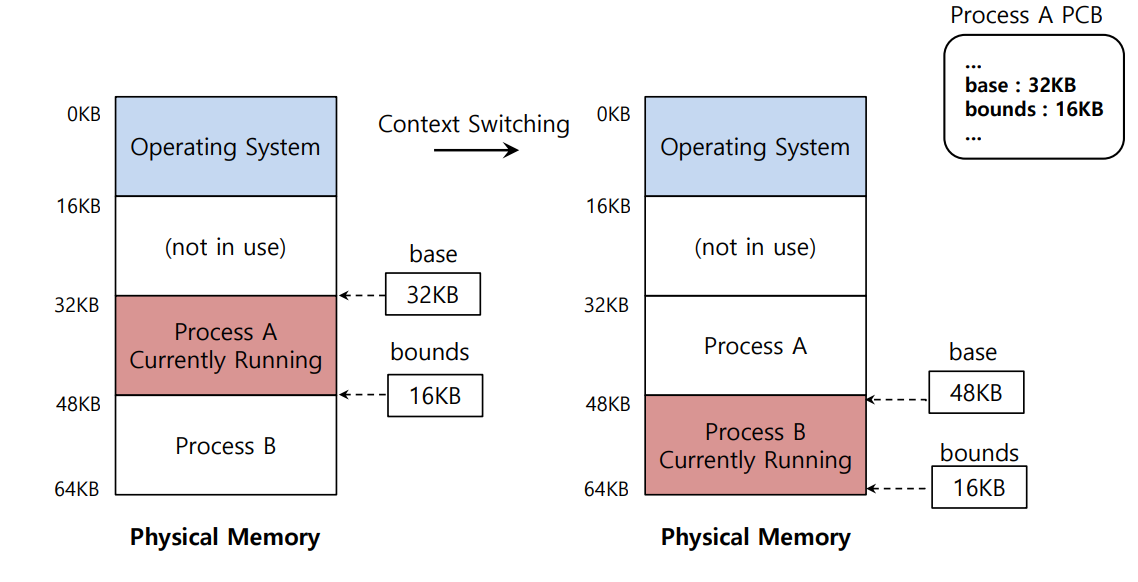
\includegraphics[width=13cm, height=6cm]{immagine_2024-11-01_160439322.png} % Percorso dell'immagine
    \caption{} % Didascalia per l'immagine
    \label{fig:immagine} % Etichetta per riferimento
\end{figure}
\vspace{100pt}
\section{Segmentazione}
\subsection{Introduzione}
L'approccio Base and Bound contiene delle inefficienze, ci sono delle grandi quantità di spazio "libero" e questo spazio "libero" prende spazio sulla memoria fisica. Inoltre è difficile da utilizzare quando uno spazio degli indirizzi non entra nella memoria fisica.
\subsection{Segmentation}
Un segmento è una porzione contigua dello spazio degli indirizzi di una determinata lunghezza. Ogni segmento può essere piazzato su differenti parti della memoria fisica, infatti Base and Bound esistono per ogni segmento. 
\begin{figure}[H] % Usa 'H' per forzare la posizione qui
    \centering % Centra l'immagine
    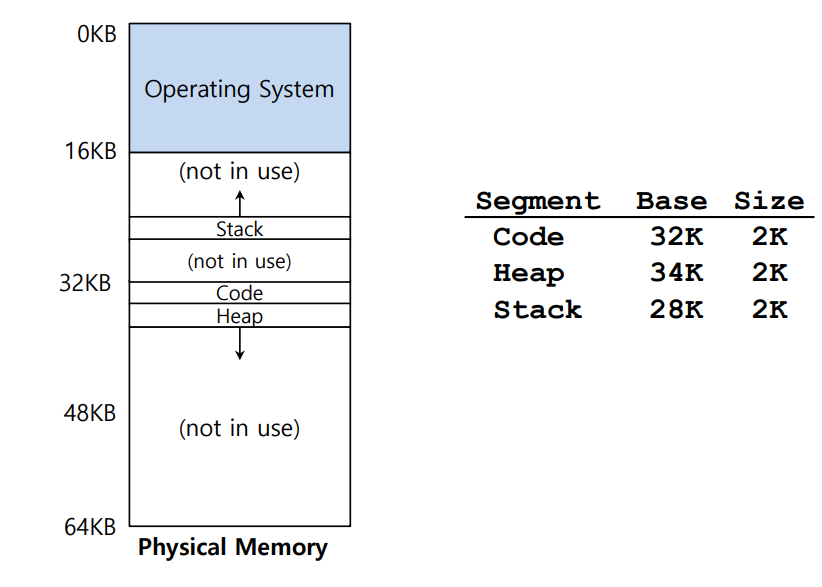
\includegraphics[width=13cm, height=6cm]{Screenshot 2024-12-09 120923.png} % Percorso dell'immagine
    \caption{} % Didascalia per l'immagine
    \label{fig:immagine} % Etichetta per riferimento
\end{figure}
\subsubsection{Traduzione degli indirizzi con la segmentazione}
$$physical\ address = offset + base$$
Dove l'offset sarebbe la posizione in cui mi trovo ora (Distanza rispetto ad una base)
\begin{figure}[H] % Usa 'H' per forzare la posizione qui
    \centering % Centra l'immagine
    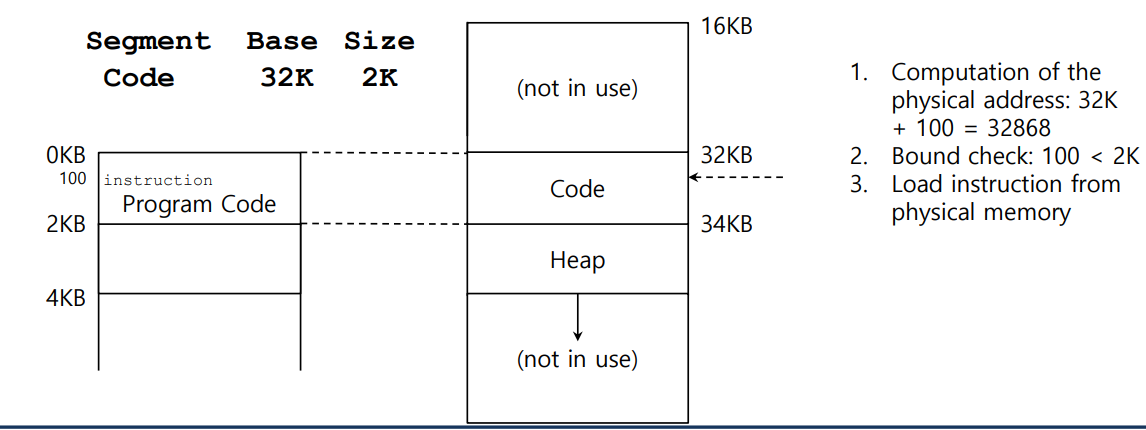
\includegraphics[width=13cm, height=5cm]{Screenshot 2024-12-09 121446.png} % Percorso dell'immagine
    \caption{} % Didascalia per l'immagine
    \label{fig:immagine} % Etichetta per riferimento
\end{figure}
\vspace{100pt}
\noindent
In questo caso l'offset è 104 perchè
$$4200 - 4096=104$$
Dove 4096 è la distanza rispetto all'inizio del segmento
\begin{figure}[H] % Usa 'H' per forzare la posizione qui
    \centering % Centra l'immagine
    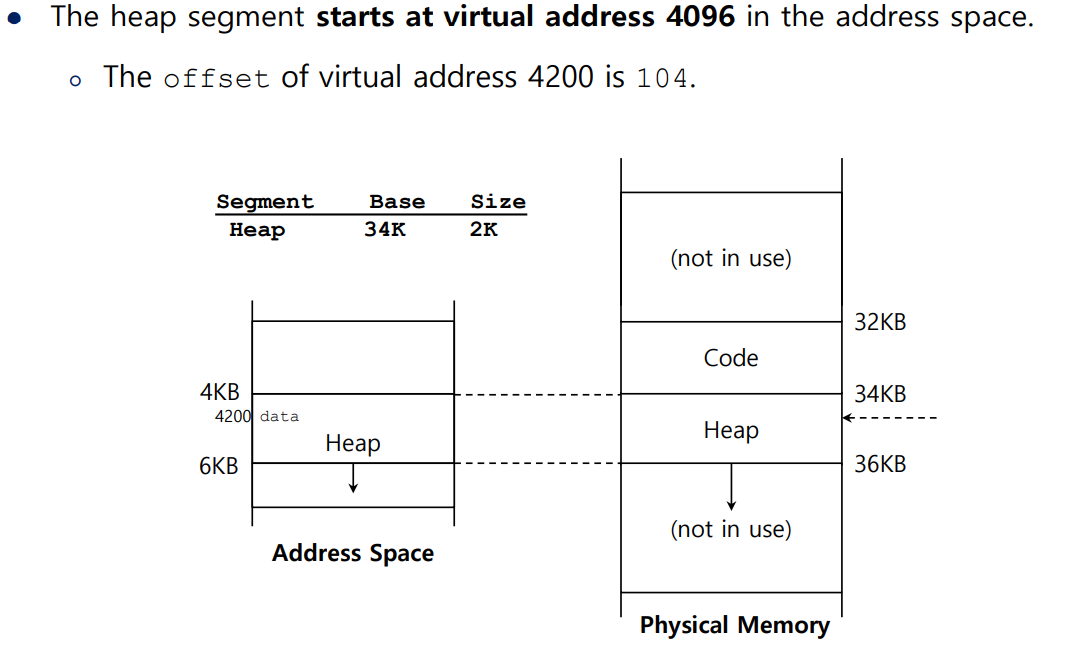
\includegraphics[width=10cm, height=5cm]{immagine_2024-12-09_121743425.png} % Percorso dell'immagine
    \caption{} % Didascalia per l'immagine
    \label{fig:immagine} % Etichetta per riferimento
\end{figure}
\subsubsection{Segmentation Fault or Violation}
Se un indirizzo non valido viene referenziato (accesso alla memoria con un puntatore o una variabile) (es. un indirizzo alla fine dell heap) la CPU lancia un eccezione e il sistema operativo manda un \textbf{segmentation fault} 
\subsubsection{Referenziare un segmento}
\textbf{Approccio esplicito} \\
Suddividere lo spazio degli indirizzi in segmenti basati sui primi (o superiori) bit dell'indirizzo virtuale. (il numero di segmenti lo sappiamo a priori, dato un indirizzo i due bit più significativi ci dicono l'indice a cui vogliamo fare riferimento)
\begin{figure}[H] % Usa 'H' per forzare la posizione qui
    \centering % Centra l'immagine
    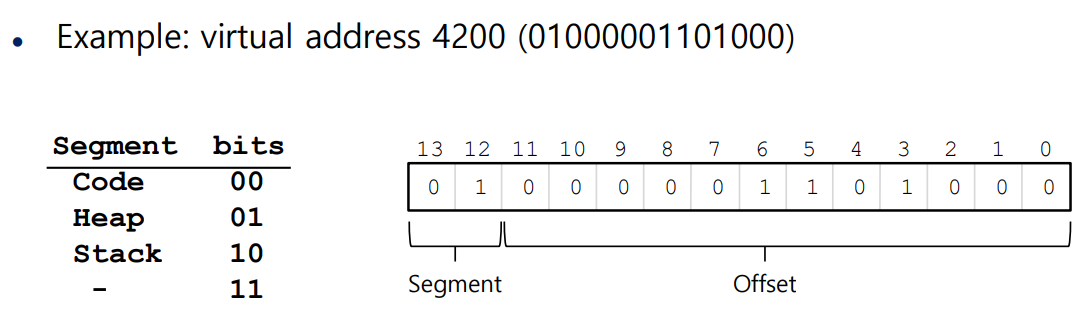
\includegraphics[width=11cm, height=3cm]{Screenshot 2024-12-09 123250.png} % Percorso dell'immagine
    \caption{} % Didascalia per l'immagine
    \label{fig:immagine} % Etichetta per riferimento
\end{figure}
\noindent
\textbf{Referenziare il segmento dello stack}\\
Lo stack cresce all'indietro per questo motivo c'è bisogno dell'aiuto dell'hardware che ci dice in che direzione sta crescendo il segmento (positiva, negativa)
\begin{figure}[H] % Usa 'H' per forzare la posizione qui
    \centering % Centra l'immagine
    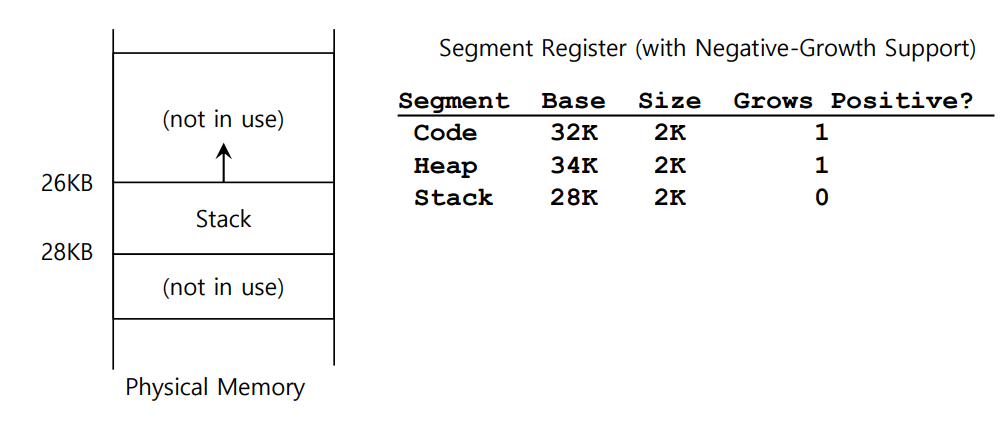
\includegraphics[width=11cm, height=3cm]{Screenshot 2024-12-09 123725.png} % Percorso dell'immagine
    \caption{} % Didascalia per l'immagine
    \label{fig:immagine} % Etichetta per riferimento
\end{figure}
I segmenti possono essere condivisi nello spazio degli indirizzi, per questo motivo grazie sempre all'aiuto dell hardware vengono inseriti altri bit per indicare i permessi.
\begin{figure}[H] % Usa 'H' per forzare la posizione qui
    \centering % Centra l'immagine
    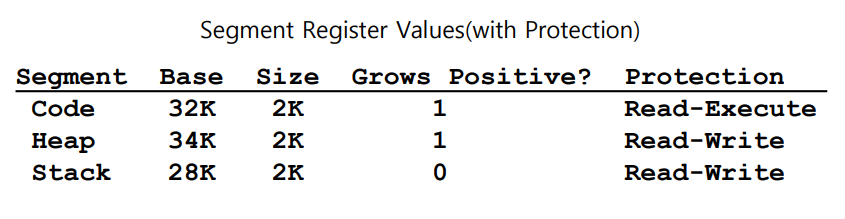
\includegraphics[width=11cm, height=3cm]{immagine_2024-12-09_124107964.png} % Percorso dell'immagine
    \caption{} % Didascalia per l'immagine
    \label{fig:immagine} % Etichetta per riferimento
\end{figure}
\subsubsection{Segmentazione a grana grossa e a grana fina}
Per\textbf{segmentazione a grana grossa} si intende un piccolo numero di grandi segmenti, i suoi pro sono: è facile da realizzare con poco hardware aggiuntivo (registri base/bound). I suoi contro sono: questo tipo di segmentazione è soggetta a frammentazione interna ovvero ho dei grandi buchi di memoria libera e dati sparsi che non posso utilizzare perchè non ne conosco il contenuto.
\\
Per \textbf{segmentazione a grana fina} intendiamo un grande numero di piccoli segmenti. I suoi pro sono: viene limitata la frammentazione interna. I suoi contro sono: un numero predefinito di registri base/bound non è abbastanza per la sua realizzazione
\subsection{Frammentazione}
\subsubsection{Frammentazione esterna}
Piccoli buchi di spazi di memoria liberi nella memoria fisica che rendono difficile l'allocazione di nuovi segmenti. Ad esempio di sono 24Kb di memoria libera ma non in un segmento unico, il sistema operativo non puo soddisfare una richiesta da 20Kb
\subsubsection{Compattazione}
Riarrangiamento dei segmenti esistenti nella memoria fisica, ed è utile per massimizzare la memoria disponibile in modo contiguo
\subsection{Come risolvere gli esercizi sulla segmentazione}
\begin{figure}[H] % Usa 'H' per forzare la posizione qui
    \centering % Centra l'immagine
    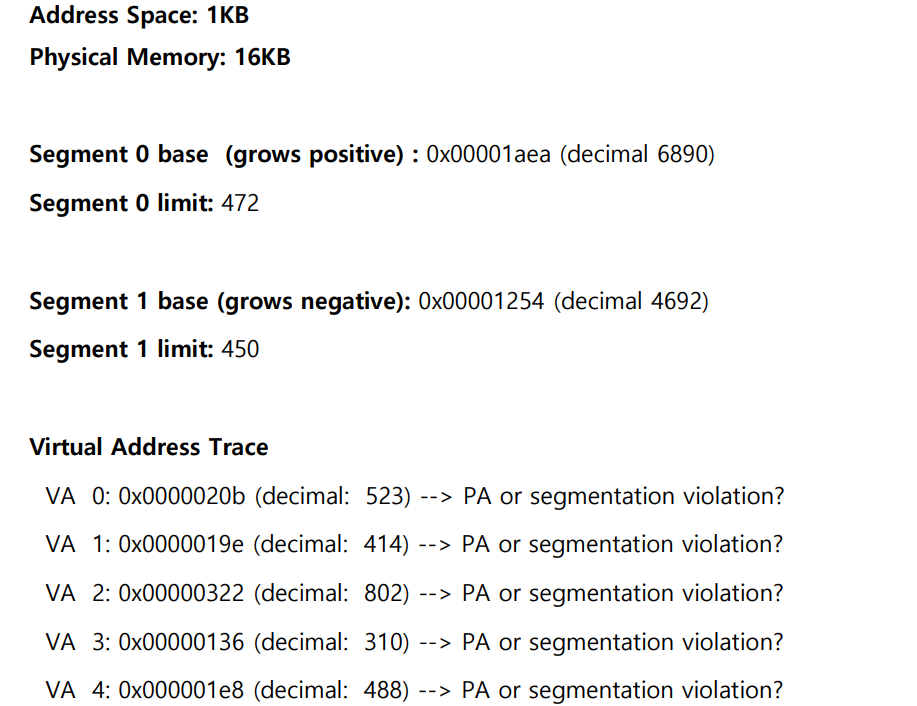
\includegraphics[width=10cm, height=6cm]{immagine_2024-12-09_132028904.png} % Percorso dell'immagine
    \caption{} % Didascalia per l'immagine
    \label{fig:immagine} % Etichetta per riferimento
\end{figure}
\noindent
La prima cosa utile da fare è disegnare lo spazio degli indirizzi e la memoria fisica.
\begin{figure}[H]
    \centering
    \begin{minipage}{0.4\textwidth} % Imposta la larghezza della colonna sinistra
        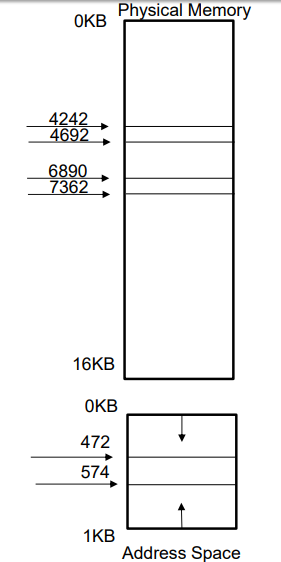
\includegraphics[width=5cm, height=10cm]{Screenshot 2024-12-09 134843.png}
        \label{fig:immagine}
    \end{minipage}%
    \hfill
    \begin{minipage}{0.55\textwidth} % Imposta la larghezza della colonna destra
       Ora ci occupiamo di tradurre gli indirizzi, cerco di capire com'è strutturato lo spazio degli indirizzi, in questo caso abbiamo il segmento 0 che cresce positivamente e ha limite 472, quindi possiamo iniziare lo spazio degli indirizzi da 0 e fermarci a 472. Il segmento 1 invece cresce negativamente, infatti quello che facciamo è
       posizionarci alla fine dello spazio degli indirizzi (grande 1kb) e calcolare dov'è posizionata la fine del segmento (grazie al limite che ci ha imposto il problema) $1024 - 450=574$. Ora per quanto riguarda la memoria fisica la disegno della giusta dimensione, e posiziono i segmenti, il calcolo è simile a prima, infatti il segmento 1 cresce positivamente, parte da 6890 a cui sommiamo 472, quindi la fine del segmento 0 sarà $6890 + 472=7362$, l'intervallo che va da 6890 a 7362 rappresenta il segmento 0. Il segmento 1 invece cresce negativamente quindi posizioniamo sulla memoria fisica 4692 a cui sottraiamo 450, quindi la fine del segmento 1 sarà $4692 - 450=4242$, l'intervallo che va da 4242 a 4692 rappresenta il segmento 1. Una volta fatti i grafici la traduzione è molto semplice. Se l'indirizzo decimale si trova in una porzione utilizzabile dello spazio degli indirizzi si passa alla traduzione. Se l'indirizzo si trova in un segmento che cresce positivamente gli si aggiunge la base al VA decimale. Se l'indirizzo si trova in un segmento che cresce negativamente alla sua base in questo caso (1024) gli si toglie l'indirizzo decimale, cosi trovando il numero da sottrarre alla base della memoria fisica per trovare il suo indirizzo in memoria fisica.

    \end{minipage}
\end{figure}
\section{Paging}
\subsection{Introduzione}
La segmentazione è utilizzata per dividere lo spazio degli indirizzi di un'applicazione in più pezzi. Uno dei problemi della segmentazione è la frammentazione della memoria. Il paging suddivide lo spazio degli indirizzi in unità di dimensione fissa chiamate pagine. Con il paging la memoria fisica è divisa in un certo numero di pagine chiamate page frame. Il problema che stiamo cercando di risolvere è come tradurre efficientemente un virtual page number (VPN) nella sua corrispondente page frame number (PFN).
\subsubsection{Vantaggi del paging}
Uno dei vantaggi del paging è la \textbf{flessibilità}: supporta efficacemente l'astrazione dello spazio degli indirizzi, non serve sapere come l'heap o lo stack crescono e come vengono utilizzati. \textbf{Semplicità}: Facilità nella gestione dello spazio libero. La pagina nello spazio degli indirizzi e il page frame sono della stessa dimensione.
\begin{figure}[H] % Usa 'H' per forzare la posizione qui
    \centering % Centra l'immagine
    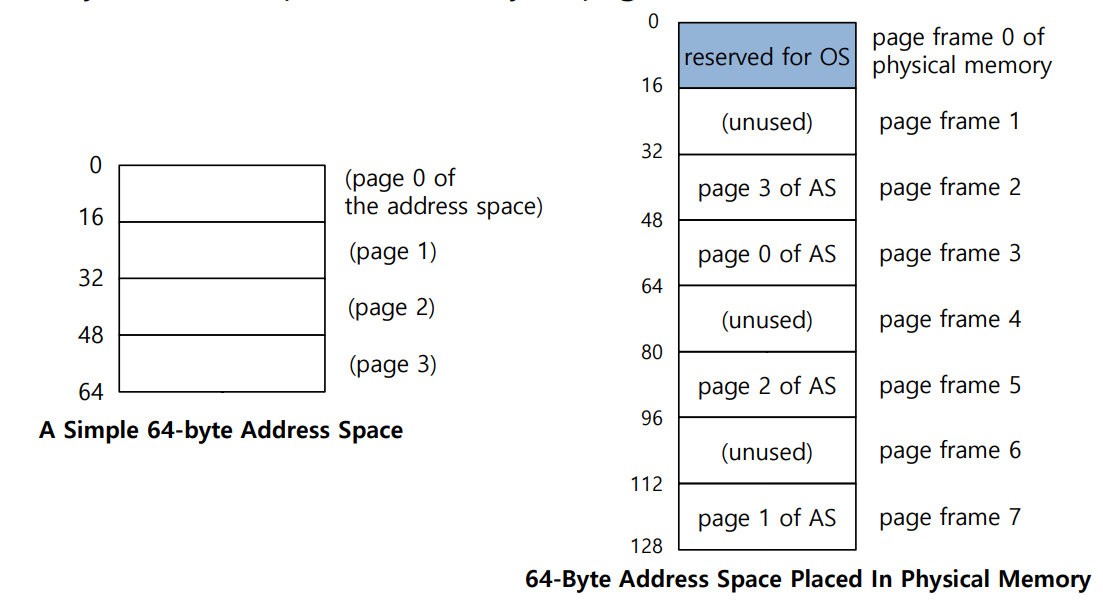
\includegraphics[width=11cm, height=6cm]{immagine_2024-12-09_145743040.png} % Percorso dell'immagine
    \caption{} % Didascalia per l'immagine
    \label{fig:immagine} % Etichetta per riferimento
\end{figure}
\noindent
\begin{figure}[H] % Usa 'H' per forzare la posizione qui
    \centering % Centra l'immagine
    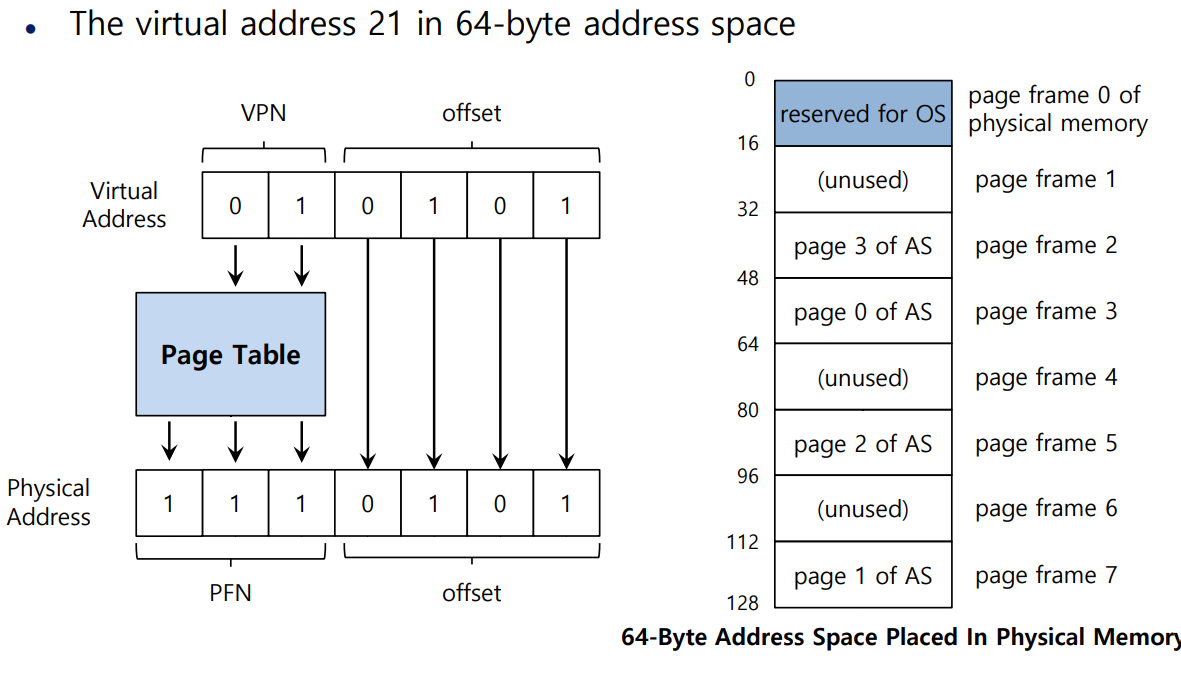
\includegraphics[width=11cm, height=6cm]{Screenshot 2024-12-09 150104.png} % Percorso dell'immagine
    \caption{} % Didascalia per l'immagine
    \label{fig:immagine} % Etichetta per riferimento
\end{figure}
\subsection{Page Table}
La page table è una struttura dati che viene utilizzata per mappare un indirizzo virtuale in uno fisico. Il sistema operativo indicizza l'array tramite il VPN e cerca la voce nella tabella delle pagine.
\begin{figure}[H] % Usa 'H' per forzare la posizione qui
    \centering % Centra l'immagine
    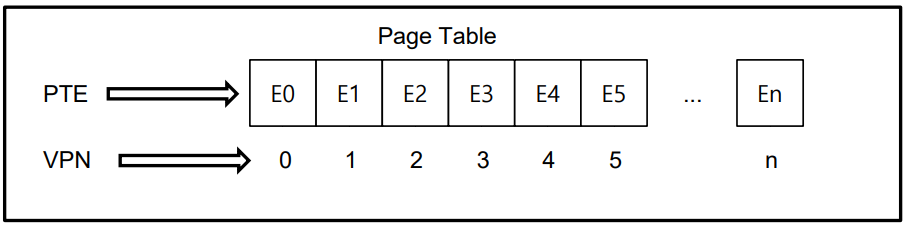
\includegraphics[width=11cm, height=3cm]{Screenshot 2024-12-09 150524.png} % Percorso dell'immagine
    \caption{} % Didascalia per l'immagine
    \label{fig:immagine} % Etichetta per riferimento
\end{figure}
\subsubsection{Contenuto della PTE}
All'interno della PTE troviamo: \textbf{Page Frame Number}: il numero della page frame nella memoria fisica. \textbf{Valid Bit}: Indicano se la traduzione è valida. \textbf{Protection Bits}: Indicano i permessi della pagina. \textbf{Present Bit}: Indicano se il contenuto della pagina si trova nella memoria fisica o su un disco. \textbf{Dirty Bit}: Indicano se la pagina è stata modificata da quando è nella memoria. \textbf{Reference Bit}: indicano se la pagina è stata acceduta.
\begin{figure}[H] % Usa 'H' per forzare la posizione qui
    \centering % Centra l'immagine
    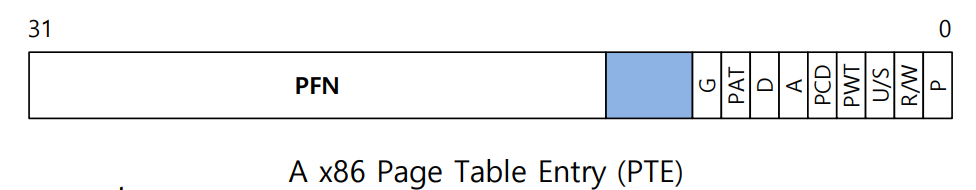
\includegraphics[width=11cm, height=2cm]{Screenshot 2024-12-09 151359.png} % Percorso dell'immagine
    \caption{} % Didascalia per l'immagine
    \label{fig:immagine} % Etichetta per riferimento
\end{figure}
\noindent
Le page table possono essere veramente grandi e facendo due calcoli occuperebbero troppo spazio. 
\begin{figure}[H] % Usa 'H' per forzare la posizione qui
    \centering % Centra l'immagine
    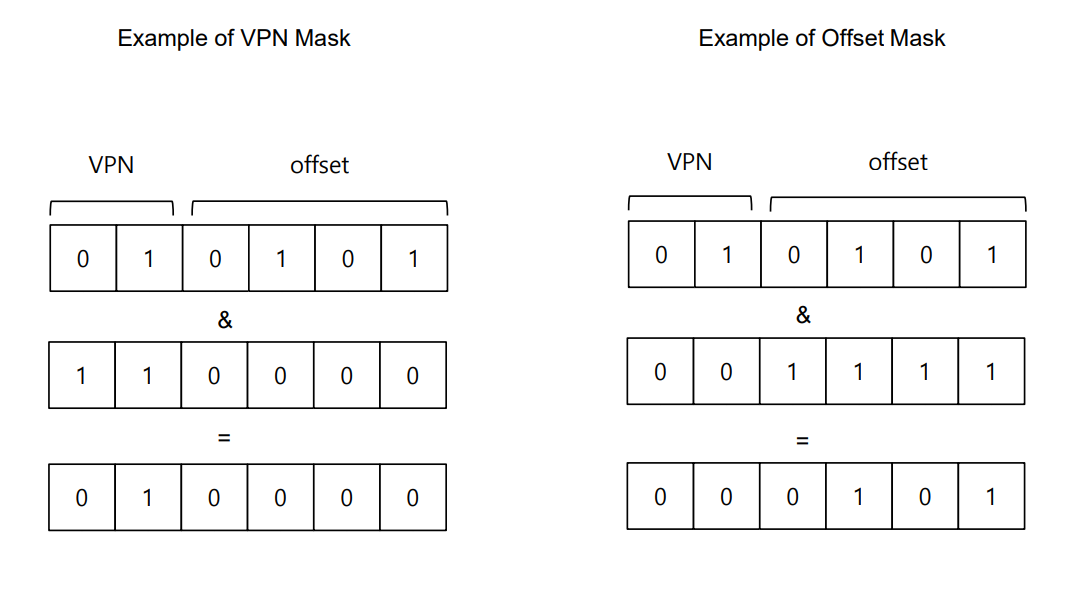
\includegraphics[width=11cm, height=6cm]{Screenshot 2024-12-09 151948.png} % Percorso dell'immagine
    \caption{} % Didascalia per l'immagine
    \label{fig:immagine} % Etichetta per riferimento
\end{figure}
\noindent
\subsection{Accesso alla memoria col paging}
\begin{figure}[H] % 'h' per indicare di posizionare la figura qui
    \centering % Centra l'intera figura
    % Immagine di sinistra
    \begin{subfigure}[t]{0.45\textwidth} % Sottotitolo di dimensione 45% della larghezza
        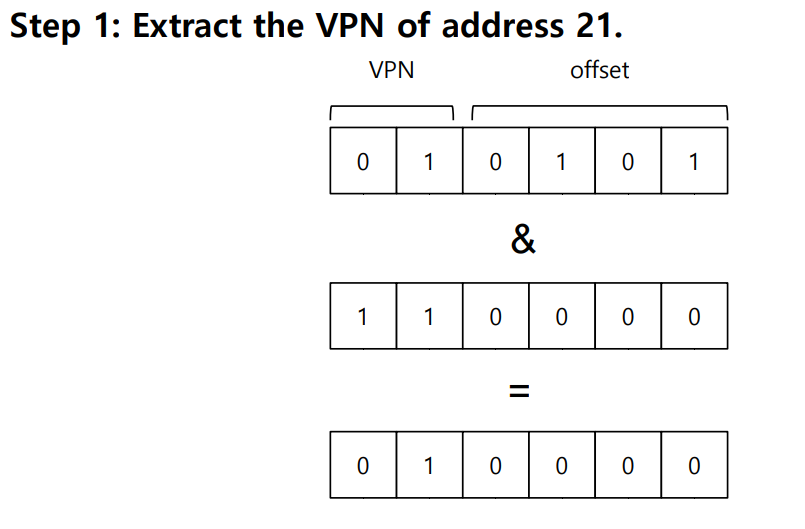
\includegraphics[width=\linewidth]{Screenshot 2024-12-09 152329.png} % Percorso dell'immagine
       % \caption{Arrivo in precedenza dei processi più piccoli} % Didascalia per la prima immagine
        \label{fig:sinistra} % Etichetta per riferimento
    \end{subfigure}
    \hspace{0.05\textwidth} % Spazio orizzontale tra le immagini
    % Immagine di destra
    \begin{subfigure}[t]{0.45\textwidth} % Sottotitolo di dimensione 45% della larghezza
        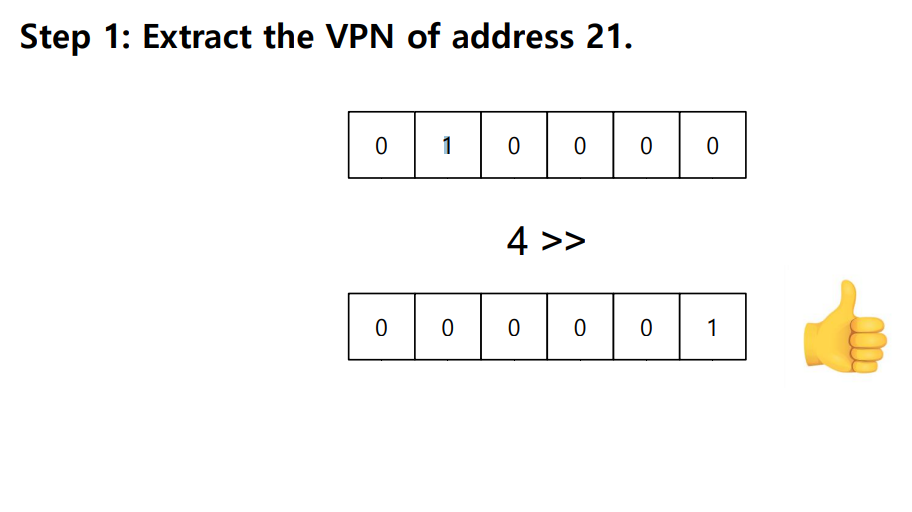
\includegraphics[width=\linewidth]{Screenshot 2024-12-09 152554.png} % Percorso dell'immagine
       % \caption{Arrivo in precedenza del processo più grande} % Didascalia per la seconda immagine
        \label{fig:destra} % Etichetta per riferimento
    \end{subfigure}
   % \caption{SJF/Shortest Job First} % Didascalia generale per la figura
    \label{fig:due_immagini} % Etichetta generale per riferimento
\end{figure}
\begin{figure}[H] % 'h' per indicare di posizionare la figura qui
    \centering % Centra l'intera figura
    % Immagine di sinistra
    \begin{subfigure}[t]{0.45\textwidth} % Sottotitolo di dimensione 45% della larghezza
        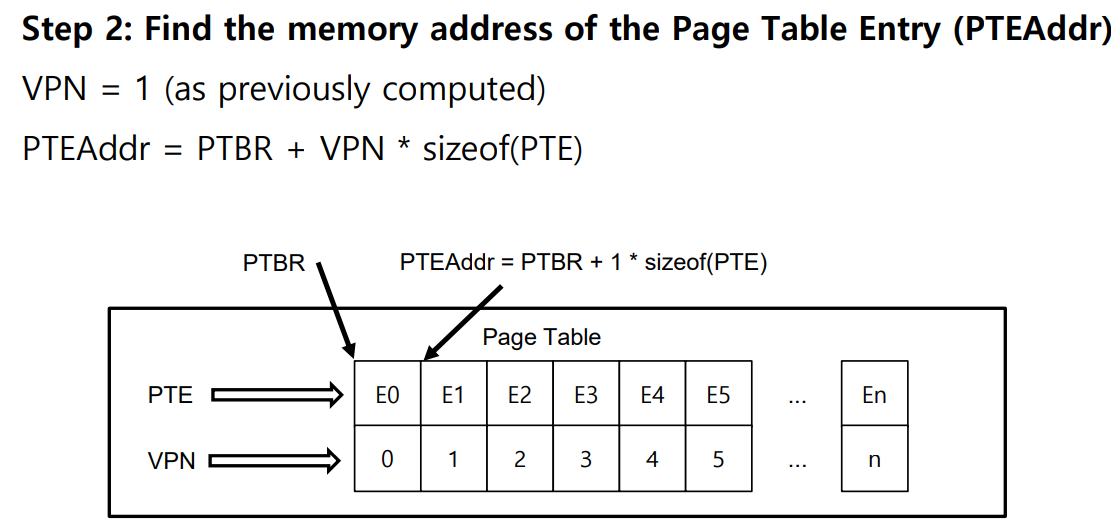
\includegraphics[width=\linewidth]{Screenshot 2024-12-09 153247.png} % Percorso dell'immagine
       % \caption{Arrivo in precedenza dei processi più piccoli} % Didascalia per la prima immagine
        \label{fig:sinistra} % Etichetta per riferimento
    \end{subfigure}
    \hspace{0.05\textwidth} % Spazio orizzontale tra le immagini
    % Immagine di destra
    \begin{subfigure}[t]{0.45\textwidth} % Sottotitolo di dimensione 45% della larghezza
        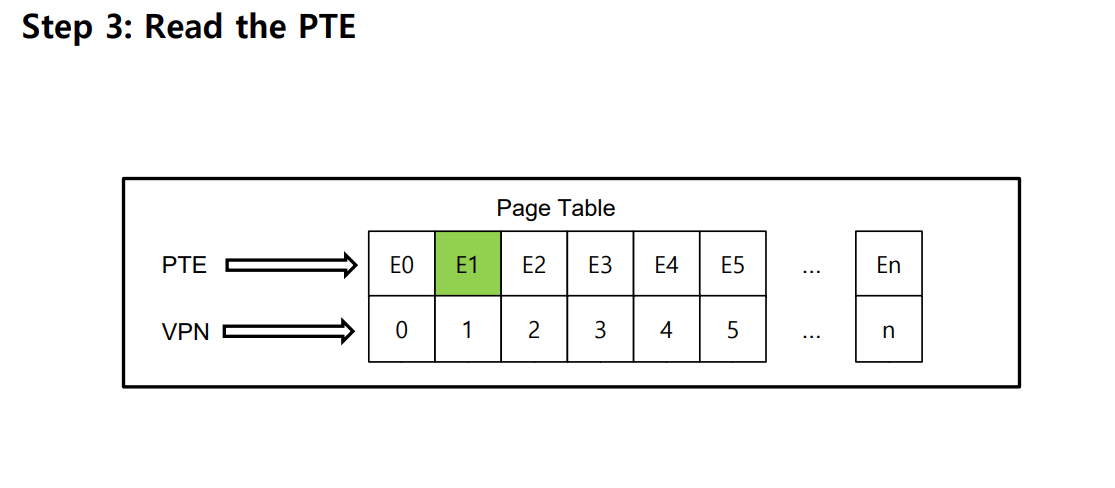
\includegraphics[width=\linewidth]{Screenshot 2024-12-09 153256.png} % Percorso dell'immagine
       % \caption{Arrivo in precedenza del processo più grande} % Didascalia per la seconda immagine
        \label{fig:destra} % Etichetta per riferimento
    \end{subfigure}
   % \caption{SJF/Shortest Job First} % Didascalia generale per la figura
    \label{fig:due_immagini} % Etichetta generale per riferimento
\end{figure}
\begin{figure}[H] % 'h' per indicare di posizionare la figura qui
    \centering % Centra l'intera figura
    % Immagine di sinistra
    \begin{subfigure}[t]{0.45\textwidth} % Sottotitolo di dimensione 45% della larghezza
        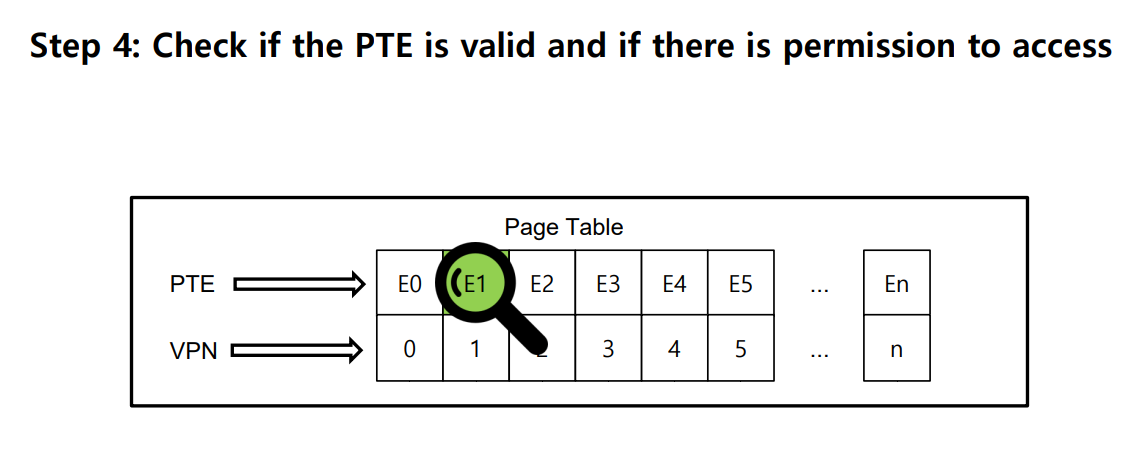
\includegraphics[width=\linewidth]{Screenshot 2024-12-09 153531.png} % Percorso dell'immagine
       % \caption{Arrivo in precedenza dei processi più piccoli} % Didascalia per la prima immagine
        \label{fig:sinistra} % Etichetta per riferimento
    \end{subfigure}
    \hspace{0.05\textwidth} % Spazio orizzontale tra le immagini
    % Immagine di destra
    \begin{subfigure}[t]{0.45\textwidth} % Sottotitolo di dimensione 45% della larghezza
        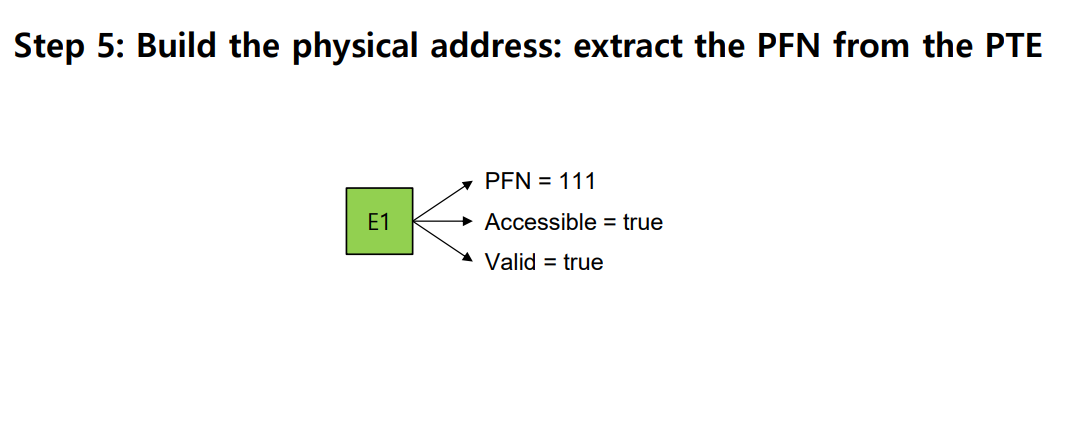
\includegraphics[width=\linewidth]{Screenshot 2024-12-09 153546.png} % Percorso dell'immagine
       % \caption{Arrivo in precedenza del processo più grande} % Didascalia per la seconda immagine
        \label{fig:destra} % Etichetta per riferimento
    \end{subfigure}
   % \caption{SJF/Shortest Job First} % Didascalia generale per la figura
    \label{fig:due_immagini} % Etichetta generale per riferimento
\end{figure}
\begin{figure}[H] % 'h' per indicare di posizionare la figura qui
    \centering % Centra l'intera figura
    % Immagine di sinistra
    \begin{subfigure}[t]{0.45\textwidth} % Sottotitolo di dimensione 45% della larghezza
        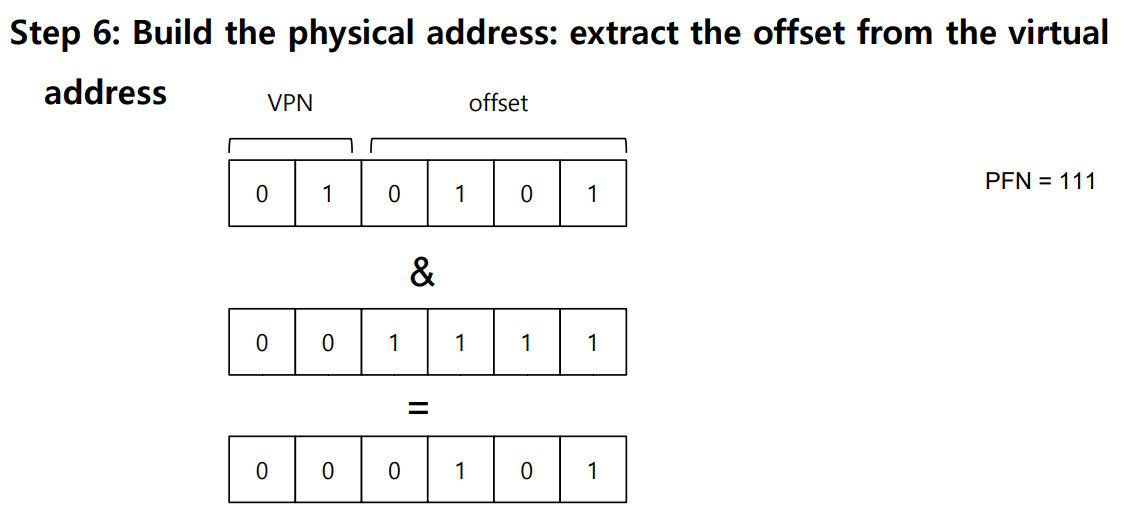
\includegraphics[width=\linewidth]{Screenshot 2024-12-09 153731.png} % Percorso dell'immagine
       % \caption{Arrivo in precedenza dei processi più piccoli} % Didascalia per la prima immagine
        \label{fig:sinistra} % Etichetta per riferimento
    \end{subfigure}
    \hspace{0.05\textwidth} % Spazio orizzontale tra le immagini
    % Immagine di destra
    \begin{subfigure}[t]{0.45\textwidth} % Sottotitolo di dimensione 45% della larghezza
        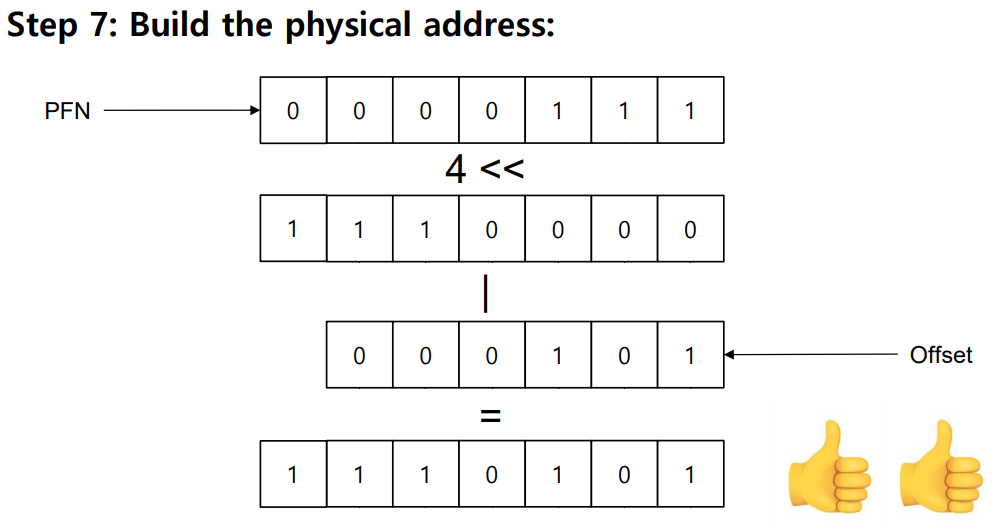
\includegraphics[width=\linewidth]{Screenshot 2024-12-09 153804.png} % Percorso dell'immagine
       % \caption{Arrivo in precedenza del processo più grande} % Didascalia per la seconda immagine
        \label{fig:destra} % Etichetta per riferimento
    \end{subfigure}
   % \caption{SJF/Shortest Job First} % Didascalia generale per la figura
    \label{fig:due_immagini} % Etichetta generale per riferimento
\end{figure}
\begin{figure}[H] % Usa 'H' per forzare la posizione qui
    \centering % Centra l'immagine
    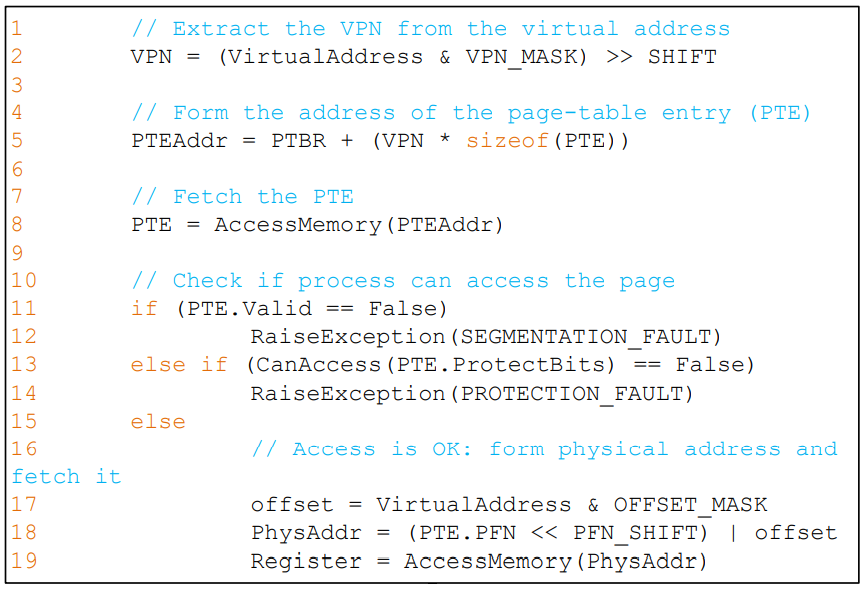
\includegraphics[width=11cm, height=6cm]{Screenshot 2024-12-09 154022.png} % Percorso dell'immagine
    \caption{} % Didascalia per l'immagine
    \label{fig:immagine} % Etichetta per riferimento
\end{figure}
\subsection{Come risolvere gli esercizi sul paging}
\begin{figure}[H]
    \centering
    \begin{minipage}{0.4\textwidth} % Imposta la larghezza della colonna sinistra
        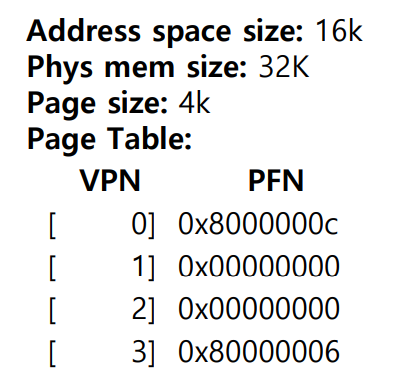
\includegraphics[width=5cm, height=6cm]{Screenshot 2024-12-09 154603.png}
        \label{fig:immagine}
    \end{minipage}%
    \hfill
    \begin{minipage}{0.55\textwidth} % Imposta la larghezza della colonna destra
       Per prima cosa osserviamo la page table, se il bit più significativo della PFN è 1 allora il resto della voce è il PFN, se è 0 la pagina non è valida. Successivamente dobbiamo ragionare sullo spazio degli indirizzi, divido il nostro indirizzo per la dimensione di una pagina (in questo caso 4096) per sapere in che pagina si trova. Se la pagina è valida, trovo l'offset che è uguale all'$offset=indirizzo - pagina\ in \ cui \ si \ trova*dimensione \ pagina$ moltiplico il pfn per la dimensione di una pagina (4096) e gli sommo l offset per trovare il PA

    \end{minipage}
\end{figure}
\begin{figure}[H] % Usa 'H' per forzare la posizione qui
    \centering % Centra l'immagine
    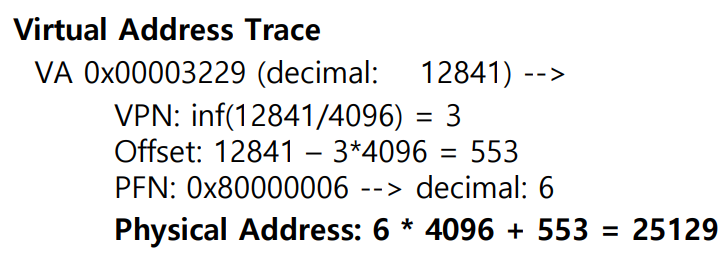
\includegraphics[width=10cm, height=4cm]{Screenshot 2024-12-09 155939.png} % Percorso dell'immagine
    \caption{} % Didascalia per l'immagine
    \label{fig:immagine} % Etichetta per riferimento
\end{figure}
\section{TLB (Translation Lookaside Buffer)}

\end{document}
